\documentclass[10pt]{article}
\usepackage[letterpaper,left=2.0cm,right=2.0cm,top=2.0cm,bottom=2.0cm]{geometry}
\setlength{\parskip}{1.6ex}
\setlength{\parindent}{0ex}
\usepackage[english]{babel}
\usepackage{times, epsfig, subfigure, psfrag, amssymb, amsmath, amsbsy, amsfonts}
\usepackage{graphicx}
\usepackage{float}
\usepackage{tabularx}
\usepackage{url}
\usepackage[utf8]{inputenc}
\usepackage[T1]{fontenc}
\usepackage{stfloats}
\usepackage{array}
\usepackage{xcolor}
\usepackage{siunitx}
\usepackage{caption}
\captionsetup{font=footnotesize,labelfont=bf,skip=4pt,hypcap=false}
\usepackage{fancyhdr}
\usepackage{datetime,enumitem}
\usepackage{algorithmic}
\usepackage{algorithm}
\usepackage{textcomp}
\usepackage{hyperref}
\usepackage{mathtools}
\usepackage{paralist}
\usepackage{multirow}
\usepackage{multicol}
\usepackage{booktabs}
\usepackage{threeparttable}
\usepackage{amsthm}
\usepackage{placeins}
\definecolor{darkgreen}{RGB}{0,100,0}
\setlist[enumerate]{topsep=0pt,parsep=0pt,partopsep=0pt}
\usepackage[nobottomtitles*]{titlesec}
\titleformat{\section}{\bfseries\large}{}{0.0em}{}[]
\titlespacing*{\section}{0cm}{2.2ex plus 0.2ex minus 0.2ex}{0.6ex plus 0.2ex minus 0.2ex}
\usepackage{ifthen}
\newcommand{\query}[2][]{\ifthenelse{\equal{#1}{}}{}{\textbf{#1:}~}\emph{#2}}
\newcommand{\ans}[1]{\textbf{Answer:~}#1}
\newcommand{\Rtext}[1]{\textbf{Revised Text:~}#1}
\newcommand{\com}[1]{\textcolor{blue}{#1}}
\newcommand{\norm}[1]{\left\|#1\right\|}

\title{Integrating Fundamental Knowledge and Sensor Data: Physics-Informed Neural Networks for Smart Agricultural Water Management: Answers to Reviewers' Comments}
\date{\today}

\begin{document}
\renewcommand{\figurename}{Fig.}
\sloppy
\begin{center}
\textbf{\Large Answers to Reviewers' and Editor's Comments and Suggestions}
\end{center}
\vspace{0.3cm}
\noindent
\textbf{Title: Integrating Fundamental Knowledge and Sensor Data: Physics-Informed Neural Networks for Smart Agricultural Water Management} \\
\textbf{Submission ID: df9266f4-d2fd-4aa0-8ca7-115166eb6609 (Scientific Reports)} \\
\textbf{Authors: Gregory Conde$^{1}$, Sandra M. Guzm\'an$^{1}$, Jorge I. Poveda$^{2}$, Flavia T. Zambon$^{3}$} \\
\textbf{Affiliations:} \\
$^{1}$Agricultural and Biological Engineering, Indian River Research and Education Center, University of Florida, Fort Pierce, FL, USA \\
$^{2}$Department of Electrical and Computer Engineering, University of California, San Diego, CA, USA \\
$^{3}$Institute of Food and Agricultural Sciences, Indian River Research and Education Center, University of Florida, Fort Pierce, FL, USA \\
\textbf{Emails: gregory.condemen@ufl.edu, sandra.guzmangut@ufl.edu, jipoveda@ucsd.edu, f.zambon@ufl.edu} \\
\vspace{0.1cm}
\setcounter{page}{1}

\textcolor{blue}{We sincerely thank the Editor and Reviewers for their thoughtful, constructive feedback, which has substantially improved the clarity, rigor, and balance of our manuscript. Below, we respond to every comment point by point, providing a concise explanation followed by the verbatim revised text and the new or updated tables and figures incorporated into the manuscript. All revisions in the enclosed tracked manuscript (\texttt{PINN\_revised\_commented.pdf}) are highlighted in blue and indexed in the margins (\texttt{E-1.1} to \texttt{E-1.2}, \texttt{R-1.1} to \texttt{R-1.10}, and \texttt{R-2.1} to \texttt{R-2.12}).}

\section*{Answers to Editor}

\textcolor{blue}{We are grateful to Assistant Editor Stefi Sebastian and Academic Editor Jianglong Shen for handling our submission and providing clear editorial guidance.}

\query[E-1.1]{\textbf{Reporting of results, claims, and limitations:} Please ensure the results are accurately reported, any overstated conclusions are rewritten and the limitations of the work fully explained. When your revision is ready, please submit the updated manuscript and a point-by-point response. This will help us move to a swift decision.}\\
\ans{\textcolor{blue}{Thank you for this guidance. We verified all reported metrics from the trained model, tempered claims across the Abstract, Introduction, Results, and Conclusions, and stated all scope boundaries explicitly: (i) exact verified metrics are reported consistently across the Abstract, Section~1, and Table~2 (overall RMSE of \SI{1.16}{\%VWC} / $\approx\SI{3.19}{mm}$ in training and \SI{1.23}{\%VWC} / $\approx\SI{3.22}{mm}$ in the 72~\si{h} forecast, with errors of $\approx\SI{1.05}{}$ to \SI{1.11}{mm} at 15 to 25~\si{cm} and $\approx\SI{0.28}{mm}$ at 35~\si{cm}); (ii) sweeping Introduction claims were replaced with a balanced comparison (Table~1), and the Abstract, Introduction, and Section~1.1 note that unconstrained ODEs can match passive 3-day RMSE ($0.97$ to \SI{1.13}{\%VWC}) while inverting physical sensitivities on $20.7\%$ to $73.4\%$ of unseen states; (iii) negative single-layer $R^2$ values on low-variance deep layers are explained mathematically alongside parity scatterplots (Fig.~3), and inferred depletion $pc_i$ ($S_i$) is qualified as total $ET_0$-driven drying rather than isolated root uptake (Section~1.2); and (iv) the dedicated Conclusions section details single-site sandy Alfisol validation, observed weather inputs, factory probe calibration, duration-based irrigation sensing, \SI{1}{h} topsoil smoothing, and the distinction between our validated open-loop estimator and future closed-loop MPC trials.}}\\
\Rtext{\emph{\textcolor{darkgreen}{Several limitations define the scope of this study and guide future work. Calibration and validation reflect a single sandy Alfisol citrus block over a 35-day training period and a 33-day spring test period using observed station meteorology, factory probe calibration, and duration-based irrigation sensing; extending the approach to finer-textured soils, other crops, live numerical weather forecasts, and site-specific volumetric calibration requires multi-site, multi-season trials. In addition, the \SI{1}{h} sampling interval matched to forecast providers smooths rapid sub-hourly infiltration peaks in sandy topsoil. Finally, the present work validates an open-loop multi-depth estimator rather than a closed-loop controller; coupling this estimator with operational weather forecasts in field model predictive control trials to measure actual water and nutrient savings is the natural next step.}}}

\query[E-1.2]{\textbf{Code availability and persistent repository deposition:} Please note that if your manuscript uses any custom or bespoke computational tool or code, or reports a new algorithm, tool, software, or a pipeline (even if individual components are not new), the underlying code must be deposited in a recognised DOI-assigning repository (e.g. zenodo) and linked either from Methods or a dedicated Code Availability section.}\\
\ans{\textcolor{blue}{Thank you for noting this requirement. We have added dedicated \textbf{Code availability} and \textbf{Data availability} sections (along with \textbf{Author contributions} and \textbf{Competing interests} statements) linking the complete Python/TensorFlow two-stage PINN pipeline, branched flux networks, \texttt{float64} RK4 solver, trained weights, field datasets, and benchmark/ablation scripts openly in Zenodo (\url{https://doi.org/10.5281/zenodo.19446129}).}}\\
\Rtext{\emph{\textcolor{darkgreen}{\textbf{Code availability:} All custom Python/TensorFlow code developed for this study, including the two-stage PINN training pipeline, branched flux-network definitions, custom \texttt{float64} RK4 solver, inference scripts, trained model weights, statistical verification utilities, and the complete benchmark, ablation, and physical admissibility evaluation scripts, is openly deposited in Zenodo at \url{https://doi.org/10.5281/zenodo.19446129}.\\
\textbf{Data availability:} The complete raw and hourly processed field sensor datasets (weather station, multi-depth soil moisture probe, and irrigation conductance telemetry) supporting all training, 3-day benchmark, and rolling unseen-window analyses are publicly deposited in Zenodo at \url{https://doi.org/10.5281/zenodo.19446129}.}}}

\query[E-1.3]{\textbf{Major revision and point-by-point response (Academic Editor):} We have received two reviews of your manuscript. Both reviewers find the topic relevant and potentially valuable. However, based on their comments, the manuscript requires major revision. Please respond to all reviewer comments point by point, provide detailed explanations of the changes made, and highlight the modifications in the revised manuscript. We look forward to receiving your revised and improved manuscript.}\\
\ans{\textcolor{blue}{We thank the Academic Editor for coordinating the review process. Every editorial and reviewer comment is addressed point by point below, including the new and updated tables (Tables~1 to 3) and figures (Figs.~1 to 7), with all manuscript additions highlighted in blue and cross-referenced in the margins of the tracked manuscript.}}

\section*{Answers to Reviewer 1}

\query[R-1.General]{The manuscript ``Integrating Fundamental Knowledge and Sensor Data: Physics-Informed Neural Networks for Smart Agricultural Water Management'' investigates the problem of making informed irrigation decisions using Physics-Informed Machine Learning techniques to predict when and where plants require water, integrating present soil moisture data with weather forecasts and irrigation history. The topic is relevant, addressing the real problem of intelligent and informed water usage. The authors report good results in terms of generalization and prediction power of their algorithm, making it suitable to estimate soil water content of crops on a 3D grid and thus make informed decisions and planning for irrigation. The manuscript is very good overall, but I would like to highlight some weak spot, concern, or curiosity, that may help. Particularly, I would suggest a revision regarding the positioning relative to previous work, the definition and interpretation of the analysed quantities, and the absence of suitable benchmark and ablation comparisons.}\\
\ans{\textcolor{blue}{We sincerely thank Reviewer~1 for the encouraging assessment of our work and for the constructive critiques regarding related literature, metric definitions and millimeter error scale, and benchmark and ablation testing. We have thoroughly revised the manuscript to address every point below.}}

\subsection*{Major Comments}

\query[R-1.1]{\textbf{State of the art and related works:} Since the ultimate goal of the manuscript is, roughly, to estimate soil water content and irrigate accordingly, a more thorough literature review would provide a more fair context and a better baseline and help the reader better understand where this paper stands, and where it shines. For example, you state that ``current approaches cannot integrate real-time soil moisture data, weather forecasts, and plant water demands into models capable of predictive control,'' but this seems to be too strong, also in light of reference~15 that you cite some paragraph later. Indeed, ref.~15 considers as ``input features for the UQ models'' ``DOY, precipitation, past SWC measurements, and residual errors from the preceding seven days'' for ``irrigation scheduling''. This content seems in contradiction with your statement ``current approaches cannot integrate real-time soil moisture data, weather forecasts, and plant water demands into models capable of predictive control'' and later ``However, none of these efforts have integrated plant, soil, and water dynamics with crop-specific sensor data to enable optimal irrigation decisions.''}\\
\ans{\textcolor{blue}{Thank you for catching this overstatement and apparent contradiction. We removed the claims that existing methods ``cannot integrate'' soil moisture, weather, and crop demand, explicitly recognized recent ML/UQ scheduling, multi-depth forecasting, physics-informed Richards' surrogates, physics-guided sequence/assimilation models, and lumped water-balance controllers~\cite{Zou2010, Murcia2024, Bagheri2025, condeforecast2024, Bandai2022, Lan2024, Elkha2024, Bandai2024, Ye2025, WangY2023, ZhangT2025, Jiang2025, Jiang2026}, and added \textbf{Table~1} comparing prior modeling families across the five core requisites needed for multi-depth predictive irrigation management.}}\\
\Rtext{\emph{\textcolor{darkgreen}{Smart irrigation systems, which utilize sensors and algorithms to optimize water delivery, offer a solution; however, while recent machine-learning, time-series, and lumped water-balance frameworks already integrate historical soil water content (SWC), weather variables, and uncertainty estimates for soil moisture forecasting and irrigation scheduling~\cite{Zou2010, Murcia2024, Bagheri2025, condeforecast2024}, achieving multi-depth root-zone resolution while preserving physical consistency for model predictive control (MPC) remains an open challenge. [...] Physics-informed neural networks (PINNs) provide the mechanism to enable the transition from passive soil moisture tracking to models capable of supporting robust model predictive control (MPC), which requires satisfying five requisites simultaneously (Table~1): multi-depth sensor resolution, learning without prescribed soil-retention curves, explicit irrigation and weather inputs, interpretable layer-by-layer water dynamics, and physically valid multi-day responses to control and weather inputs. Existing studies satisfy only subsets of these requisites across three spaces: physics-informed Richards' surrogates~\cite{Bandai2022, Lan2024, Elkha2024, Bandai2024, Ye2025} omit crop sinks and irrigation control inputs; data-driven and physics-guided forecasters~\cite{Zou2010, Murcia2024, Bagheri2025, WangY2023, ZhangT2025, Jiang2025, Jiang2026} lack decomposed fluxes and physical response guarantees under sparse field data; and control-oriented water-balance models~\cite{condeforecast2024} lump the root zone into a single layer.}}}

\begin{center}
\begin{minipage}{0.98\linewidth}
\centering
\renewcommand{\theHtable}{r1.\arabic{table}}
\setcounter{table}{0}
\captionof{table}{\textcolor{blue}{(Revised manuscript) Comparison of modeling families against the five core requisites for multi-depth predictive irrigation management.}}
\scriptsize
\setlength{\tabcolsep}{3.5pt}
{\color{blue}\begin{tabular*}{\linewidth}{@{\extracolsep{\fill}}>{\raggedright\arraybackslash}p{0.27\linewidth}>{\raggedright\arraybackslash}p{0.16\linewidth}ccccc@{}}
\toprule
\textbf{Modeling Family} & \textbf{Studies} & \textbf{Multi-} & \textbf{No Soil-} & \textbf{Explicit} & \textbf{Depth} & \textbf{Physically} \\
 & & \textbf{Depth} & \textbf{Curve} & \textbf{Irrig.} & \textbf{Fluxes \&} & \textbf{Consistent} \\
 & & \textbf{Profile} & \textbf{Calib.} & \textbf{Input} & \textbf{Depletion} & \textbf{Control} \\
\midrule
Analytical Richards' PDE models & \cite{Celia1990, swap2024} & $\checkmark$ & $\times$ & $\checkmark$ & $\checkmark$ & Partial$^{\mathrm{a}}$ \\
Physics-informed PDE \& operator surrogates & \cite{Bandai2022, Lan2024, Elkha2024, Bandai2024, Ye2025} & $\checkmark$ & Partial & $\times$ & $\times$ & $\times$ \\
Data-driven time-series \& ML forecasters & \cite{Zou2010, Murcia2024, Bagheri2025} & Partial & $\checkmark$ & $\times$ & $\times$ & $\times$ \\
Physics-guided sequence \& assimilation models & \cite{WangY2023, ZhangT2025, Jiang2025, Jiang2026} & $\checkmark$ & $\times$ & $\times$ & $\times$ & $\times$ \\
Control-oriented lumped water balance & \cite{condeforecast2024} & $\times$ & $\checkmark$ & $\checkmark$ & Partial$^{\mathrm{b}}$ & $\checkmark$ \\
\midrule
\textbf{Proposed sensor-depth PINN} & \textbf{This study} & \boldmath$\checkmark$ & \boldmath$\checkmark$ & \boldmath$\checkmark$ & \boldmath$\checkmark$ & \boldmath$\checkmark$ \\
\bottomrule
\end{tabular*}}
\vspace{2pt}
{\footnotesize\color{blue}\raggedright
$^{\mathrm{a}}$Physically consistent, but iterative nonlinear PDE solving is computationally demanding for online MPC.\par
$^{\mathrm{b}}$Separates lumped rainfall, evapotranspiration, and drainage gains, but without vertical depth localization.\par}
\end{minipage}
\end{center}

\query[R-1.2]{\textbf{Clear definitions of the considered quantities:} Greater attention to the precise definitions of quantities consider in the manuscript may help clarity and readability:
\begin{compactitem}
\item $ET_0$: evapotranspiration is never defined, and the FAO guidelines talking about it are the last reference in your manuscript. A brief introduction on its significance and the formula to compute is suggested;
\item SWC, SM, \%VWC: here the manuscript creates confusion using these overlapping terms without proper definition:
\begin{compactenum}[(a)]
\item Soil water content is used only in the introduction section with its acronym SWC;
\item Soil moisture seems to be the central metric, but its acronym SM is never introduced and appears the first time in Fig.~1;
\item \%VWC is never introduced, except as a unit of measure of soil moisture in Fig.~1.
\end{compactenum}
\end{compactitem}
I suggest to add one paragraph for each quantity, stating briefly how it is measured/computed. Most importantly, the ambiguity in the definition of \%VWC makes it a difficult metric to interpret. I discuss my concerns below.}\\
\ans{\textcolor{blue}{Thank you for pointing out these missing definitions. We now explicitly define soil moisture (SM, used interchangeably with soil water content, SWC), volumetric water content (\si{\%VWC}, liquid water volume per bulk soil volume, $\mathrm{cm^3\,cm^{-3}} \times 100$), and reference evapotranspiration ($ET_0$, \si{mm/h}, quantifying potential atmospheric evaporative demand computed from meteorological station measurements via the FAO-56 Penman--Monteith equation~\cite{allen1998crop}) in Section~1 and Section~2.3.}}\\
\Rtext{\emph{\textcolor{darkgreen}{Throughout this work, soil moisture (SM, used interchangeably with SWC) is quantified as volumetric water content (\si{\%VWC}, liquid water volume per bulk soil volume, $\mathrm{cm^3\,cm^{-3}} \times 100$), while $ET_0$ (\si{mm/h}) quantifies potential atmospheric evaporative demand via the FAO-56 Penman--Monteith equation~\cite{allen1998crop}.}}}

\query[R-1.3a]{\textbf{Interpretability of results: metric scale and error quantification (\%VWC):} Due to the ``relative'' nature of the main metric, \%VWC, the reported mean squared error will be as well relative. Without an absolute value of the errors, it may be difficult to quantify their scale. Particularly in this context, absolute errors are related to water wastage, which is a central problem in Smart Agriculture.}\\
\ans{\textcolor{blue}{This is a critical practical point. In this study, Sentek probes are operated under factory default calibration, which the manufacturer recommends for tracking relative moisture dynamics in commercial operations, where $\SI{1}{\%VWC} = \SI{0.01}{cm^3\,cm^{-3}}$ corresponds to $\approx\SI{1.0}{mm}$ of water per \SI{10}{cm} (\SI{100}{mm}) sensor layer. Over the 72~\si{h} free-run forecast, this yields per-layer RMSEs of $\approx\SI{0.28}{}$ to \SI{2.02}{mm} and a \SI{60}{cm} profile RMSE of $\approx\SI{3.22}{mm}$ ($\approx\SI{3.19}{mm}$ in training), comparable to typical capacitive probe tolerances ($\pm 1$ to \SI{2}{mm} per layer). Importantly, the largest error ($\approx\SI{2.02}{mm}$) is confined to rapid surface wetting spikes at 5~\si{cm}, while RMSE drops to $\approx\SI{1.05}{}$ to \SI{1.11}{mm} in the active root zone (15 to 25~\si{cm}) and $\approx\SI{0.28}{mm}$ at 35~\si{cm}, providing millimetric resolution right below the $\approx\SI{30}{cm}$ root zone where downward water movement represents percolation loss. We report both \si{\%VWC} and equivalent millimeter depth in Section~1 (with a concise footnote linking Sentek's \emph{Moisture Calibration Manual}), update \textbf{Table~2}, and note default factory calibration in Section~2.3.}}\\
\Rtext{\emph{\textcolor{darkgreen}{In this study, Sentek probes are used under factory calibration, where each \SI{1}{\%VWC} variation across a \SI{10}{cm} layer corresponds to $\approx\SI{1.0}{mm}$ of water.$^{1}$ Over the 72~\si{h} free-run forecast, this yields per-layer RMSEs of $\approx\SI{0.28}{}$ to \SI{2.02}{mm} and a \SI{60}{cm} profile RMSE of $\approx\SI{3.22}{mm}$ ($\approx\SI{3.19}{mm}$ in training), comparable to typical capacitive probe tolerances ($\pm 1$ to \SI{2}{mm} per layer). The largest error ($\approx\SI{2.02}{mm}$) is confined to rapid surface wetting spikes at 5~\si{cm}, while RMSE drops to $\approx\SI{1.05}{}$ to \SI{1.11}{mm} in the active root zone (15 to 25~\si{cm}) and $\approx\SI{0.28}{mm}$ at 35~\si{cm}, providing millimetric resolution right below the $\approx\SI{30}{cm}$ root zone where downward water movement represents percolation loss.\\
{\footnotesize $^{1}$Sentek recommends factory calibration for relative moisture dynamics ($\SI{1}{\%VWC} = \SI{0.01}{cm^3\,cm^{-3}}$, or \SI{1.0}{mm} of water per \SI{100}{mm} layer); see \url{https://sentektechnologies.com/download/moisture-calibration-manual/}.}}}}

\begin{center}
\begin{minipage}{0.96\linewidth}
\centering
\setcounter{table}{1}
\captionof{table}{(Revised manuscript) Statistical analysis of soil moisture estimation across six soil layers, covering training \textcolor{blue}{(35 days, $839\,\mathrm{h}$/layer)} and forecasting \textcolor{blue}{(3 days, $72\,\mathrm{h}$/layer)} periods. \textcolor{blue}{$\sigma_m$ is the measured standard deviation (\si{\%VWC}),} RMSE is the root-mean-square error in \si{\%VWC}, SD is the \textcolor{blue}{error} standard deviation, $R^2$ is the coefficient of determination\textcolor{blue}{, and $r$ is the Pearson correlation coefficient}. The obtained $p$-values indicate statistical significance ($p < 0.0001$ \textcolor{blue}{via two-sided Student's $t$-test, except $^*p = 0.0038$ at 25~\si{cm} in forecasting}). The overall result is obtained by analyzing the concatenated data from the six soil layers.}
\footnotesize
\setlength{\tabcolsep}{5.0pt}
\begin{tabular}{@{}lcccccccccc@{}}
\toprule
& \multicolumn{5}{c}{Training} & \multicolumn{5}{c}{Forecasting} \\
\cmidrule(lr){2-6}\cmidrule(l){7-11}
\textcolor{blue}{Depth} & \textcolor{blue}{$\sigma_m$} & RMSE & SD & $R^2$ & \textcolor{blue}{$r$} & \textcolor{blue}{$\sigma_m$} & RMSE & SD & $R^2$ & \textcolor{blue}{$r$} \\
\midrule
5~\si{cm}  & \textcolor{blue}{3.53} & \textcolor{blue}{1.90} & 1.81 & \textcolor{blue}{0.710} & \textcolor{blue}{0.858} & \textcolor{blue}{3.99} & \textcolor{blue}{2.02} & \textcolor{blue}{1.81} & \textcolor{blue}{0.740} & \textcolor{blue}{0.948} \\
15~\si{cm} & \textcolor{blue}{2.16} & \textcolor{blue}{0.91} & 0.90 & \textcolor{blue}{0.821} & \textcolor{blue}{0.910} & \textcolor{blue}{1.47} & \textcolor{blue}{1.11} & 0.99 & \textcolor{blue}{0.417} & \textcolor{blue}{0.802} \\
25~\si{cm} & \textcolor{blue}{1.08} & \textcolor{blue}{0.77} & 0.73 & \textcolor{blue}{0.492} & \textcolor{blue}{0.772} & \textcolor{blue}{0.87} & \textcolor{blue}{1.05} & \textcolor{blue}{0.85} & \textcolor{blue}{$-0.455$} & \textcolor{blue}{$0.337^*$} \\
35~\si{cm} & \textcolor{blue}{0.88} & \textcolor{blue}{0.45} & 0.44 & \textcolor{blue}{0.741} & \textcolor{blue}{0.888} & \textcolor{blue}{0.42} & \textcolor{blue}{0.28} & 0.24 & \textcolor{blue}{0.567} & \textcolor{blue}{0.841} \\
45~\si{cm} & \textcolor{blue}{2.14} & \textcolor{blue}{0.79} & 0.76 & \textcolor{blue}{0.865} & \textcolor{blue}{0.953} & \textcolor{blue}{0.34} & \textcolor{blue}{0.95} & \textcolor{blue}{0.49} & \textcolor{blue}{$-7.043$} & \textcolor{blue}{0.709} \\
55~\si{cm} & \textcolor{blue}{3.09} & \textcolor{blue}{1.47} & 1.40 & \textcolor{blue}{0.772} & \textcolor{blue}{0.934} & \textcolor{blue}{0.17} & \textcolor{blue}{1.32} & 0.64 & \textcolor{blue}{$-59.517$} & \textcolor{blue}{0.713} \\
\midrule
Overall & \textcolor{blue}{2.56} & \textcolor{blue}{1.16} & 1.12 & \textcolor{blue}{0.796} & \textcolor{blue}{0.901} & \textcolor{blue}{2.81} & \textcolor{blue}{1.23} & \textcolor{blue}{1.24} & \textcolor{blue}{0.807} & \textcolor{blue}{0.921} \\
\bottomrule
\end{tabular}
\end{minipage}
\end{center}

\query[R-1.3b]{\textbf{Interpretability of results: test-set $R^2$ values vs. visual agreement in Fig.~1:} Then, the reported test-set $R^2$ values appear inconsistent with the close agreement suggested visually in Fig.~1. Please clarify how $R^2$ was calculated and explain this apparent discrepancy.}\\
\ans{\textcolor{blue}{Thank you for asking us to clarify this statistical behavior. Within individual deep layers (25, 45, and 55~\si{cm}), measured soil moisture is nearly constant during the 3-day window ($\sigma_m = 0.87$, $0.34$, and \SI{0.17}{\%VWC}). Because single-layer $R^2_i = 1 - \mathrm{MSE}_i/\sigma_{m,i}^2$ divides squared error by near-zero variance, small offset biases of \SI{0.95}{} and \SI{1.32}{\%VWC} at 45 and 55~\si{cm} produce strongly negative $R^2_i$ values ($-7.043$ and $-59.517$) despite positive Pearson correlations ($r = 0.709$ and $0.713$), whereas the Overall $R^2 = 0.807$ is computed against the full-profile variance ($\sigma_m = \SI{2.81}{\%VWC}$).}}\\
\Rtext{\emph{\textcolor{darkgreen}{Specifically, the Overall row concatenates all six depth series ($6 \times 839 = 5{,}034$ training and $6 \times 72 = 432$ forecasting points; Fig.~3) relative to the full-profile variance ($\sigma_m = \SI{2.81}{\%VWC}$), whereas within individual deep layers (25, 45, and 55~\si{cm}) 3-day moisture is nearly static ($\sigma_m = 0.87$, $0.34$, and \SI{0.17}{\%VWC}). Dividing squared error by near-zero variance ($R^2_i = 1 - \mathrm{MSE}_i/\sigma_{m,i}^2$) turns small offset biases at 45 and 55~\si{cm} (\SI{0.95}{} and \SI{1.32}{\%VWC}) into strongly negative single-layer $R^2$ values despite positive correlations ($r = 0.709$ and $0.713$). Therefore, the negative values indicate that at such depths there is low data variability and that the measured data could be better explained by the average than by the model, so overall $R^2$ should be interpreted alongside per-layer RMSE and $r$.}}}

\query[R-1.3c]{\textbf{Interpretability of results: scatterplot and data concatenation:} It would be interesting to see a scatterplot of predicted vs measured data, to understand the real capabilities of the model, along with a more thorough comment about ``the measured data could be better explained by the average than by the model''. Also, what happens when data is concatenated? And how is it concatenated?}\\
\ans{\textcolor{blue}{We appreciate this suggestion and added \textbf{Fig.~3} plotting predicted versus measured soil moisture color-coded by sensor depth across all $6 \times 839 = 5{,}034$ training points and $6 \times 72 = 432$ forecasting points. Concatenating the six depth vectors evaluates global residual error across the full vertical moisture span ($\sigma_m = \SI{2.81}{\%VWC}$), while the tight clustering of deep layers (45 to 55~\si{cm}) near the 1:1 line illustrates visually why a flat layer mean outperforms a slightly offset trajectory in $R^2_i$ when temporal variance is near zero.}}\\
\Rtext{\emph{\textcolor{darkgreen}{See revised text under R-1.3b above and the new parity scatterplot figure (Fig.~3) below.}}}

\begin{center}
\begin{minipage}{0.92\linewidth}
\centering
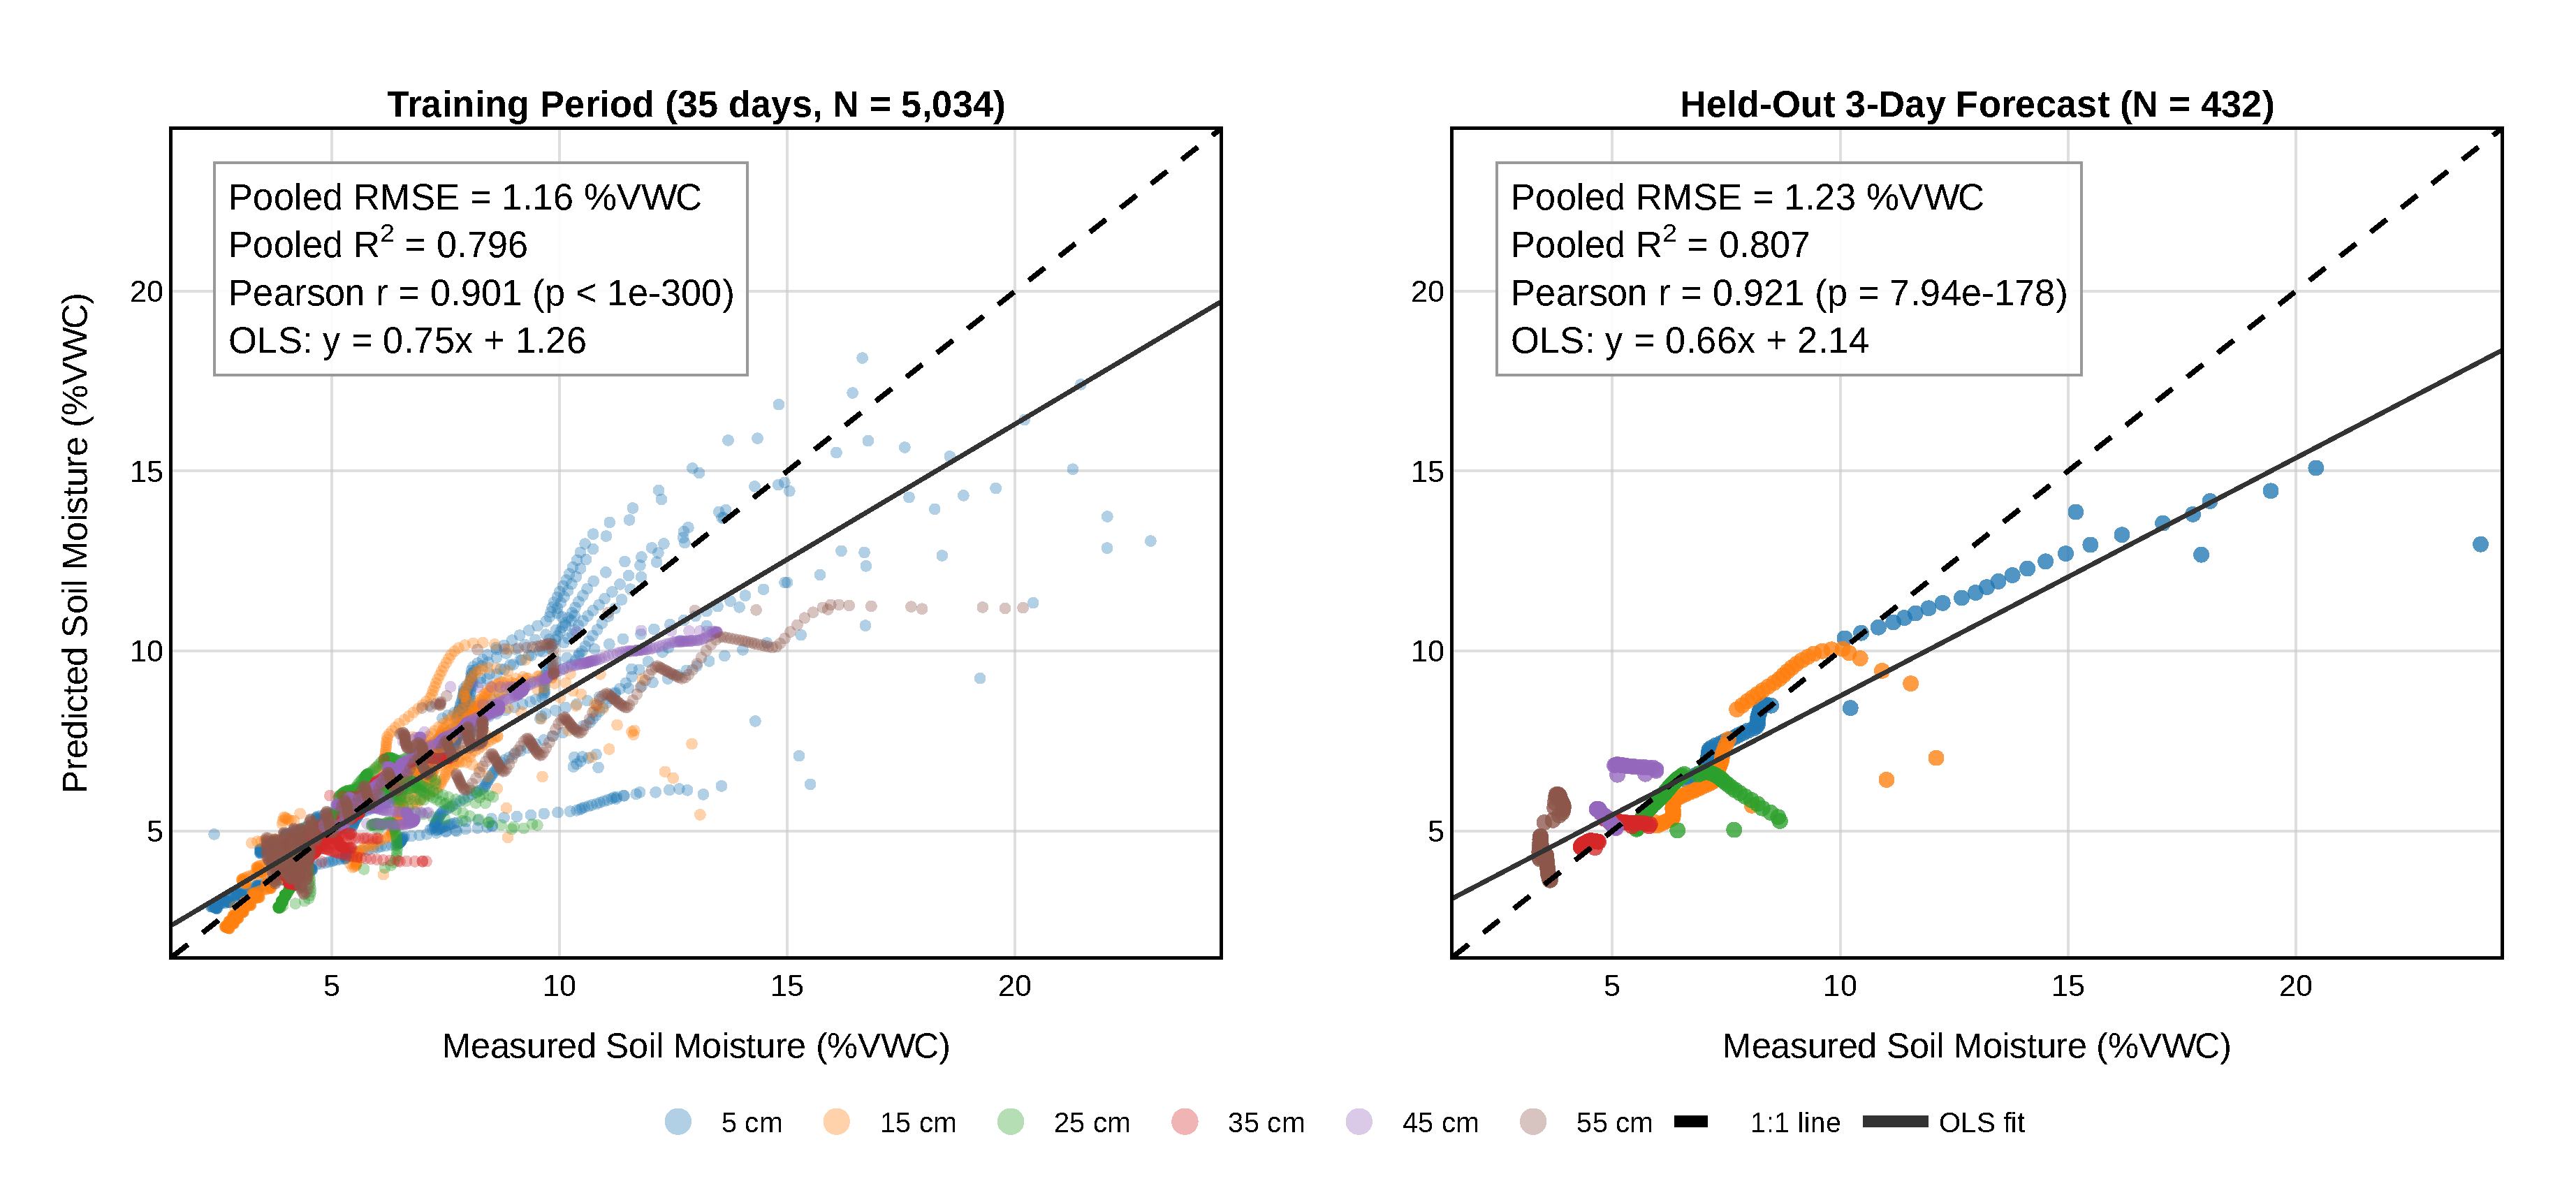
\includegraphics[width=0.95\linewidth]{predicted_vs_measured_scatter.pdf}
\setcounter{figure}{2}
\captionof{figure}{\textcolor{blue}{(Revised manuscript) Predicted versus measured soil moisture scatterplots across all six sensor depths (5--55~\si{cm}) for the 35-day training period ($N = 5{,}034$ concatenated points) and the 3-day held-out forecast ($N = 432$ points), showing tight clustering around the 1:1 line for low-variance deep layers (45--55~\si{cm}) alongside the profile-wide vertical span underlying the overall $R^2 = 0.807$ and $r = 0.921$. Dashed lines denote the 1:1 parity reference, and solid lines show the ordinary least squares (OLS) linear regression fit.}}
\end{minipage}
\end{center}

\query[R-1.3d]{\textbf{Interpretability of results: benchmark comparison, model complexity, and ablation study:} Finally, a major flaw of the manuscript is the lack of a benchmark. Indeed, the proposed algorithm is really complex, by your own words ``including numerical integration of the model in the training process significantly complicates the optimization problem''. Is this complexity justified? Are the results supported by theory? Are there other methods, either AI or not, to estimate these quantities? Is it possible to design a simpler, or more traditional, ML algorithm suited for this task? For example, does the plant uptake estimated by NNs have some reference value in literature or does it follow some rationale? Also, an ablation study removing the physics-informed terms would also help establish which components are responsible for the reported performance.}\\
\ans{\textcolor{blue}{Thank you for this foundational comment. We added Section~1.1 (\textbf{Table~3}) evaluating seven configurations across the 35-day training period, the held-out 3-day test window, 30 rolling 3-day unseen windows ($792\,\mathrm{h}$), and an automatic-differentiation derivative check ($4{,}752$ unseen state-layer points), alongside literature validation of inferred depletion in Section~1.2:
\begin{compactenum}[1.]
\item \textbf{Two-stage RK4 justification (Ablation~1):} Consistent with derivative-to-trajectory identification theory~\cite{Ribeiro2020, Aguirre2010, Bradley2021}, Stage~1 initializes $\boldsymbol{\Theta}$ in a contractive basin without integration blow-up, while Stage~2 suppresses multi-step drift. Omitting Stage~2 (\textbf{Ablation~1}) raises 3-day RMSE from \SI{1.23}{} to \SI{1.55}{\%VWC} (training: \SI{1.16}{} to \SI{2.52}{\%VWC}).
\item \textbf{Physical regularizer ablation (Ablation~2):} Removing $c_1$ to $c_3$ raises 3-day RMSE to \SI{1.39}{\%VWC} and causes 33.0\% rainfall and 42.0\% $ET_0$ derivative sign violations (26.7\% negative and 19.5\% non-monotonic branch evaluations).
\item \textbf{Simpler and unconstrained ML baselines:} The PINN cuts 3-day error by 35.6\% over \textbf{Persistence} (\SI{1.91}{} to \SI{1.23}{\%VWC}; 53.2\% in 5~\si{cm} topsoil). Although unconstrained \textbf{Linear ODE} (\SI{0.97}{\%VWC}) and \textbf{Black-Box ODEs} (\SI{1.13}{} and \SI{1.26}{\%VWC}) match passive 3-day RMSE because rain and fixed 2~\si{h} irrigations drive 96.2\% of hourly $\Delta m$ variance, they invert physical sensitivities across 20.7\% to 73.4\% of unseen states (predicting topsoil drying under irrigation on 52.9\% to 96.8\% of unseen hours), whereas the PINN maintains 0.0\% irrigation and rainfall sign inversions.
\item \textbf{Literature rationale for inferred depletion:} In Section~1.2, summed daily profile drying ($\approx\SI{2.04}{mm/d}$ in training, $\approx\SI{1.89}{mm/d}$ unseen) and the subsurface peak at 25~\si{cm} ($\approx\SI{0.28}{mm/d}$) agree with published Florida citrus spring ET ($2$ to \SI{5}{mm/d}) and feeder-root distributions ($64\%$ to $90\%$ within 0 to 30~\si{cm})~\cite{Morgan2006, Kadyampakeni2014}.
\end{compactenum}}}
\Rtext{\emph{\textcolor{darkgreen}{Both ablations confirm the design in Section~2: omitting Stage-2 trajectory refinement (\textbf{Ablation~1}) raises 3-day RMSE from 1.23 to 1.55~\si{\%VWC} (training: 1.16 to 2.52~\si{\%VWC}) due to integration drift, whereas removing the physical regularizers (\textbf{Ablation~2}) raises 3-day RMSE to 1.39~\si{\%VWC} and introduces 33.0\% rain and 42.0\% $ET_0$ sign violations, while the full PINN reduces 3-day error by 35.6\% over \textbf{Persistence} (1.91 to 1.23~\si{\%VWC}; 53.2\% in the 5~\si{cm} topsoil, from 4.32 to 2.02~\si{\%VWC}). [...] Crucially, although unconstrained \textbf{Linear ODE} ($\dot{m} = Am + Bu + c_0$) and two-stage \textbf{Black-Box ODE} ($\dot{m} = \mathrm{MLP}(m, q_{\mathrm{irr}}, r, ET_0)$) reach slightly lower passive 3-day RMSE (by 0.10 to 0.26~\si{\%VWC}), this stems from sparse field data dominated by routine wetting pulses: rain and fixed 2-hour sprinkler runs ($q_{\mathrm{irr}} \in \{0, 0.5, 1.0\}\,\si{h/h}$) account for 96.2\% of hourly $\Delta m$ variance, whereas slow daytime $ET_0$ drying accounts for only 1.6\%. Fitting historical cases alone causes unconstrained models to invert physical responses across 20.7\% to 73.4\% of unseen states, predicting soil drying under shorter irrigation doses (6 to 15~\si{min}) and root-zone wetting under high $ET_0$, with no flux or depletion curves.}}}

\begin{center}
\begin{minipage}{0.98\linewidth}
\centering
\setcounter{table}{2}
\captionof{table}{\textcolor{blue}{(Revised manuscript) Ablation and baseline comparison pairing free-run forecasting RMSE (\si{\%VWC}) with unphysical input-derivative rates across unseen field states ($792\,\mathrm{h} \times 6$ layers) and flux/depletion interpretability.}}
\scriptsize
\setlength{\tabcolsep}{2.8pt}
{\color{blue}\begin{tabular*}{\linewidth}{@{\extracolsep{\fill}}lccccccc@{}}
\toprule
 & \multicolumn{3}{c}{Free-Run RMSE (\si{\%VWC})} & \multicolumn{3}{c}{Unphysical Derivative Rate (\%)} & Flux \& \\
\cmidrule(lr){2-4}\cmidrule(lr){5-7}
Model & 35-d Train & 3-d Test & 30 Unseen 3-d & $\frac{\partial \dot{m}}{\partial q_{\mathrm{irr}}}{<}0$ & $\frac{\partial \dot{m}}{\partial r}{<}0$ & $\frac{\partial \dot{m}}{\partial ET_0}{>}0$ & Depletion \\
 & RMSE ($R^2$) & RMSE ($R^2$) & Mean$\pm$SD & (dries) & (dries) & (wets) & Curves? \\
\midrule
\multicolumn{8}{@{}l}{\textit{A. Proposed PINN and architectural ablations}} \\[1pt]
\textbf{Proposed PINN (Full)} & \textbf{1.16 (0.80)} & \textbf{1.23 (0.81)} & \textbf{1.04$\pm$0.53} & \textbf{0.0} & \textbf{0.0} & \textbf{2.5}$^\dagger$ & \textbf{Yes} \\
Ablation 1 (Stage 1 only) & 2.52 (0.03) & 1.55 (0.70) & 1.33$\pm$0.35 & 0.0 & 0.0 & 1.0 & Yes \\
Ablation 2 (Unregularized) & 1.48 (0.67) & 1.39 (0.76) & 1.00$\pm$0.30 & 0.0 & 33.0 & 42.0 & Violated$^\ddagger$ \\
\midrule
\multicolumn{8}{@{}l}{\textit{B. Reference baselines (uninterpretable or physically unconstrained)}} \\[1pt]
Persistence ($\dot{m}=0$) & 2.44 (0.09) & 1.91 (0.54) & 1.86$\pm$1.02 & --- & --- & --- & No \\
Linear State-Space ODE & 1.35 (0.72) & 0.97 (0.88) & 0.82$\pm$0.27 & 33.3 & 0.0 & 33.3 & No \\
Black-Box ODE (374k) & 0.91 (0.87) & 1.13 (0.84) & 0.98$\pm$0.57 & 70.5 (52.9$^*$) & 32.6 & 40.7 & No \\
Black-Box ODE (2.2k) & 0.85 (0.89) & 1.26 (0.80) & 1.77$\pm$2.43 & 73.4 (96.8$^*$) & 20.7 & 28.2 & No \\
\bottomrule
\end{tabular*}}
\vspace{2pt}
{\footnotesize\color{blue}\raggedright
$^*$In the 5~\si{cm} topsoil layer alone, $\partial \dot{m}_1/\partial q_{\mathrm{irr}} < 0$ occurs on 52.9\% (Black-Box 374k) and 96.8\% (Black-Box 2.2k) of unseen hours.\par
$^\dagger$Residual from soft-penalty training convergence near dry states ($\le +0.01\,\text{\%VWC/h per mm/h}$), negligible relative to sensor resolution.\par
$^\ddagger$Without physical regularizers, 26.7\% of learned branch evaluations become negative and 19.5\% violate monotonicity.\par}
\end{minipage}
\end{center}

\subsection*{Minor Comments}

\query[R-1.4]{[page 6 / page 5] An illustration of the crop configuration may help the reader better understand the data and better follow your statements ``...because the crop is in a bed with a ditch next to it, which directly evaporates water relative to $ET_0$ patterns,'' and ``The direct influence of rain at deeper layers is related to the terrain configuration''. Also the dimensions or spatial extent of the considered field are unclear.}\\
\ans{\textcolor{blue}{Thank you for this helpful suggestion. We added \textbf{Fig.~6} illustrating the raised sandy Alfisol bed, flanking drainage ditches, $\approx\SI{30}{cm}$ argillic clay horizon, under-tree micro-sprinkler, and 6-depth Sentek probe placement, while clarifying the block dimensions (35-acre research block; 20-acre active trial with 5,500 trees) in Section~2.3.}}\\
\Rtext{\emph{\textcolor{darkgreen}{This 35-acre citrus trial site is dedicated to exploring multiple breeding lines for tolerance to Huanglongbing (HLB; greening). Currently, 20 acres host a 6-year-old experiment evaluating grapefruit, grapefruit-like, sweet orange, and mandarin varieties from the University of Florida and USDA programs, grafted onto distinct rootstocks, comprising 5,500 trees across four trials. The site's Classical Alfisols are poorly drained, with a shallow sandy profile over an argillic clay horizon that limits root growth to $\approx\SI{30}{cm}$, a condition exacerbated by seawater intrusion. Trees are planted on raised beds surrounded by ditches to mitigate salinity, promote drainage, and support shallow citrus roots (Fig.~6, creating lateral subsurface drainage pathways and sloped bed shoulders exposed to direct rainfall).}}}

\begin{center}
\begin{minipage}{0.92\linewidth}
\centering
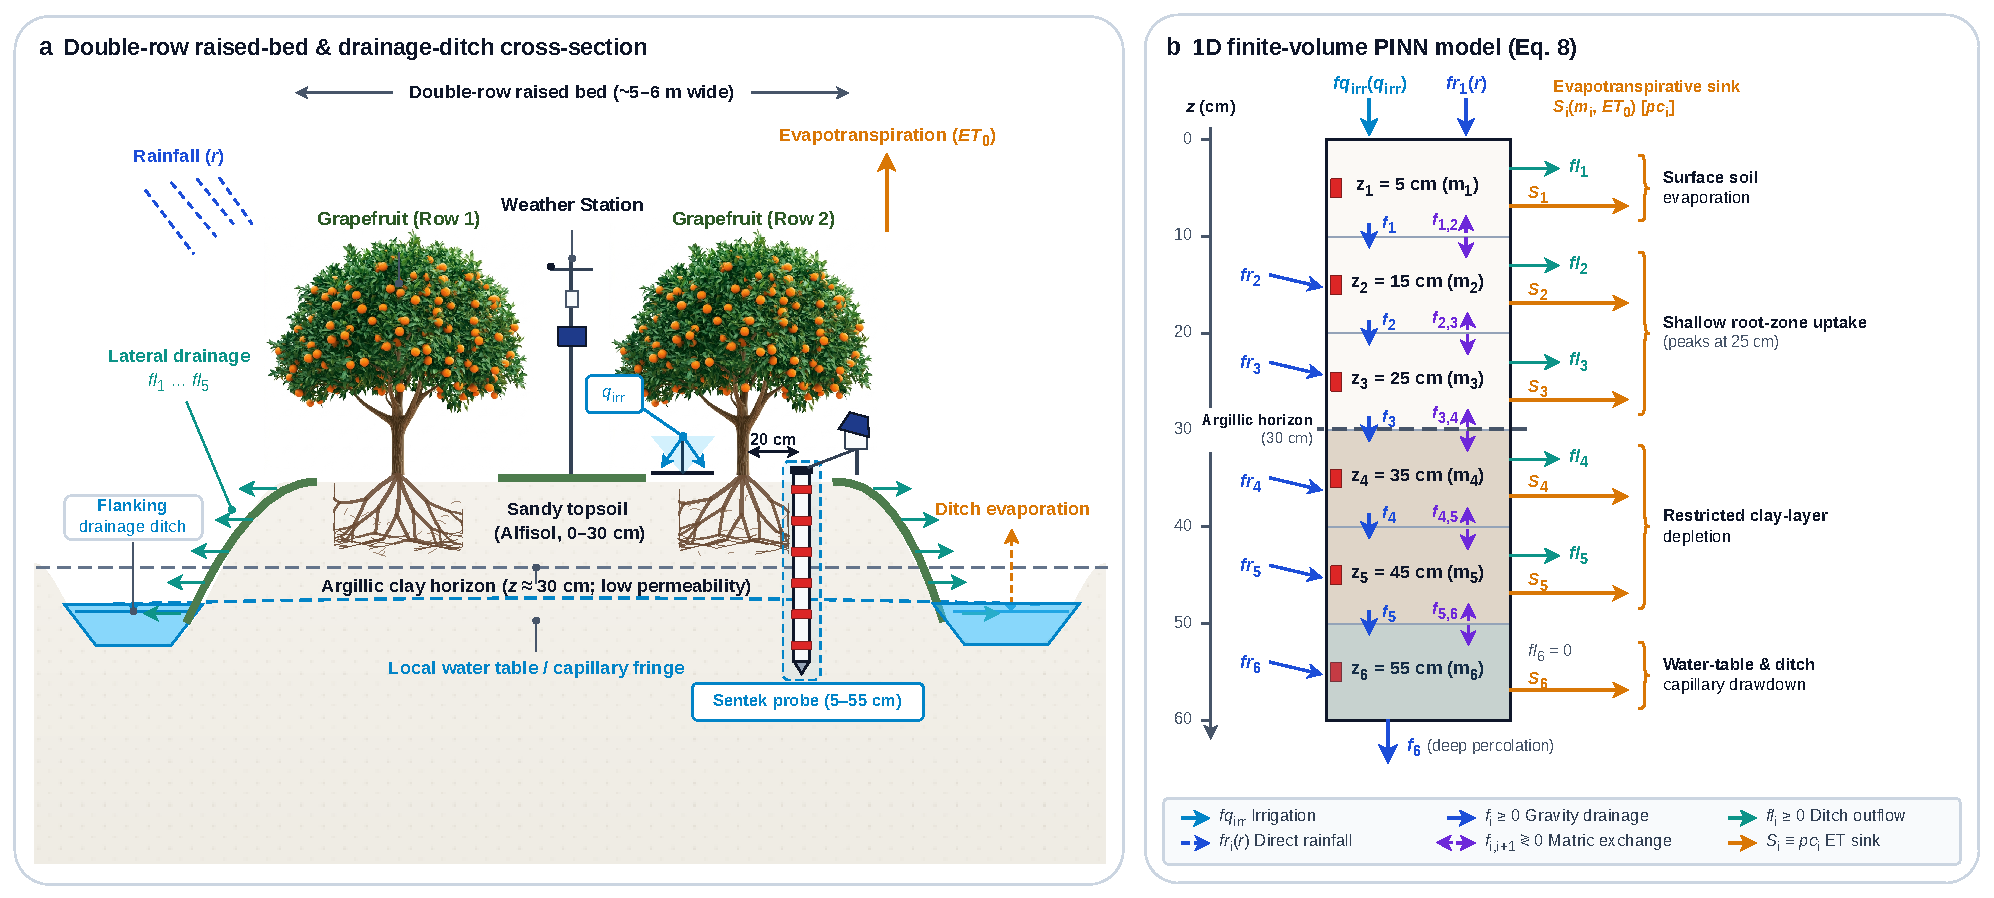
\includegraphics[width=0.92\linewidth]{bed_ditch_schematic.pdf}
\setcounter{figure}{5}
\captionof{figure}{\textcolor{blue}{(Revised manuscript) Cross-sectional geometry (not to scale) of the IRREC Millennium Block experimental site (35-acre block; 20-acre active 5,500-tree citrus trial), showing a citrus tree planted on a raised sandy Alfisol bed flanked by drainage ditches above an argillic horizon at $\approx\SI{30}{cm}$ depth. A 6-depth Sentek Drill \& Drop capacitive probe (\SI{20}{cm} from the trunk) monitors 10-\si{cm} vertical compartments centered at 5, 15, 25, 35, 45, and 55~\si{cm}, alongside micro-sprinkler irrigation ($q_{\mathrm{irr}}$), rainfall ($r$), evapotranspiration ($ET_0$), vertical percolation ($f_i$), inter-layer exchange ($f_{i,i+1}$), and lateral ditch drainage ($fl_1\dots fl_5$).}}
\end{minipage}
\end{center}

\query[R-1.5]{[page 12] The unit of irrigation flow $\mathrm{m}^3$ needs an exponentiation;}\\
\ans{\textcolor{blue}{Thank you for spotting this typo. We corrected the volumetric flow unit to \si{m^3/h} in Section~2.2.1.}}\\
\Rtext{\emph{\textcolor{darkgreen}{Specifically, $q_{\mathrm{irr}}$ is incorporated as the irrigation related variable, and $fq_{\mathrm{irr}}(q_{\mathrm{irr}})$ is a function that explains the rate of change of the soil moisture in relation to irrigation; note that $q_{\mathrm{irr}}$ could have units of flow (e.g., \si{m^3/h}) or units of relative time (e.g., \si{h/h}) indicating how much irrigation was active during a period of time.}}}

\query[R-1.6]{[fig.4] A better caption explaining all the elements of the Figure may help. The network labels and functions are not clear ($f_{i, i+1}(m_i, m_{i+1})$ should be at depth 5 and $f_i(m_i)$ at depth 2 following the first row).}\\
\ans{\textcolor{blue}{Thank you for catching both the figure label issues and the brief caption. We updated \textbf{Fig.~5} (formerly Fig.~4), correcting the branch labels and the ``Tracking Loss'' spelling and expanding the caption to define every input, neural flux branch, training stage ($j_1, j_2$), and soft penalty ($c_1$ to $c_3$).}}\\
\Rtext{\emph{\textcolor{darkgreen}{See updated Fig.~5 and its expanded caption below.}}}

\begin{center}
\begin{minipage}{0.92\linewidth}
\centering
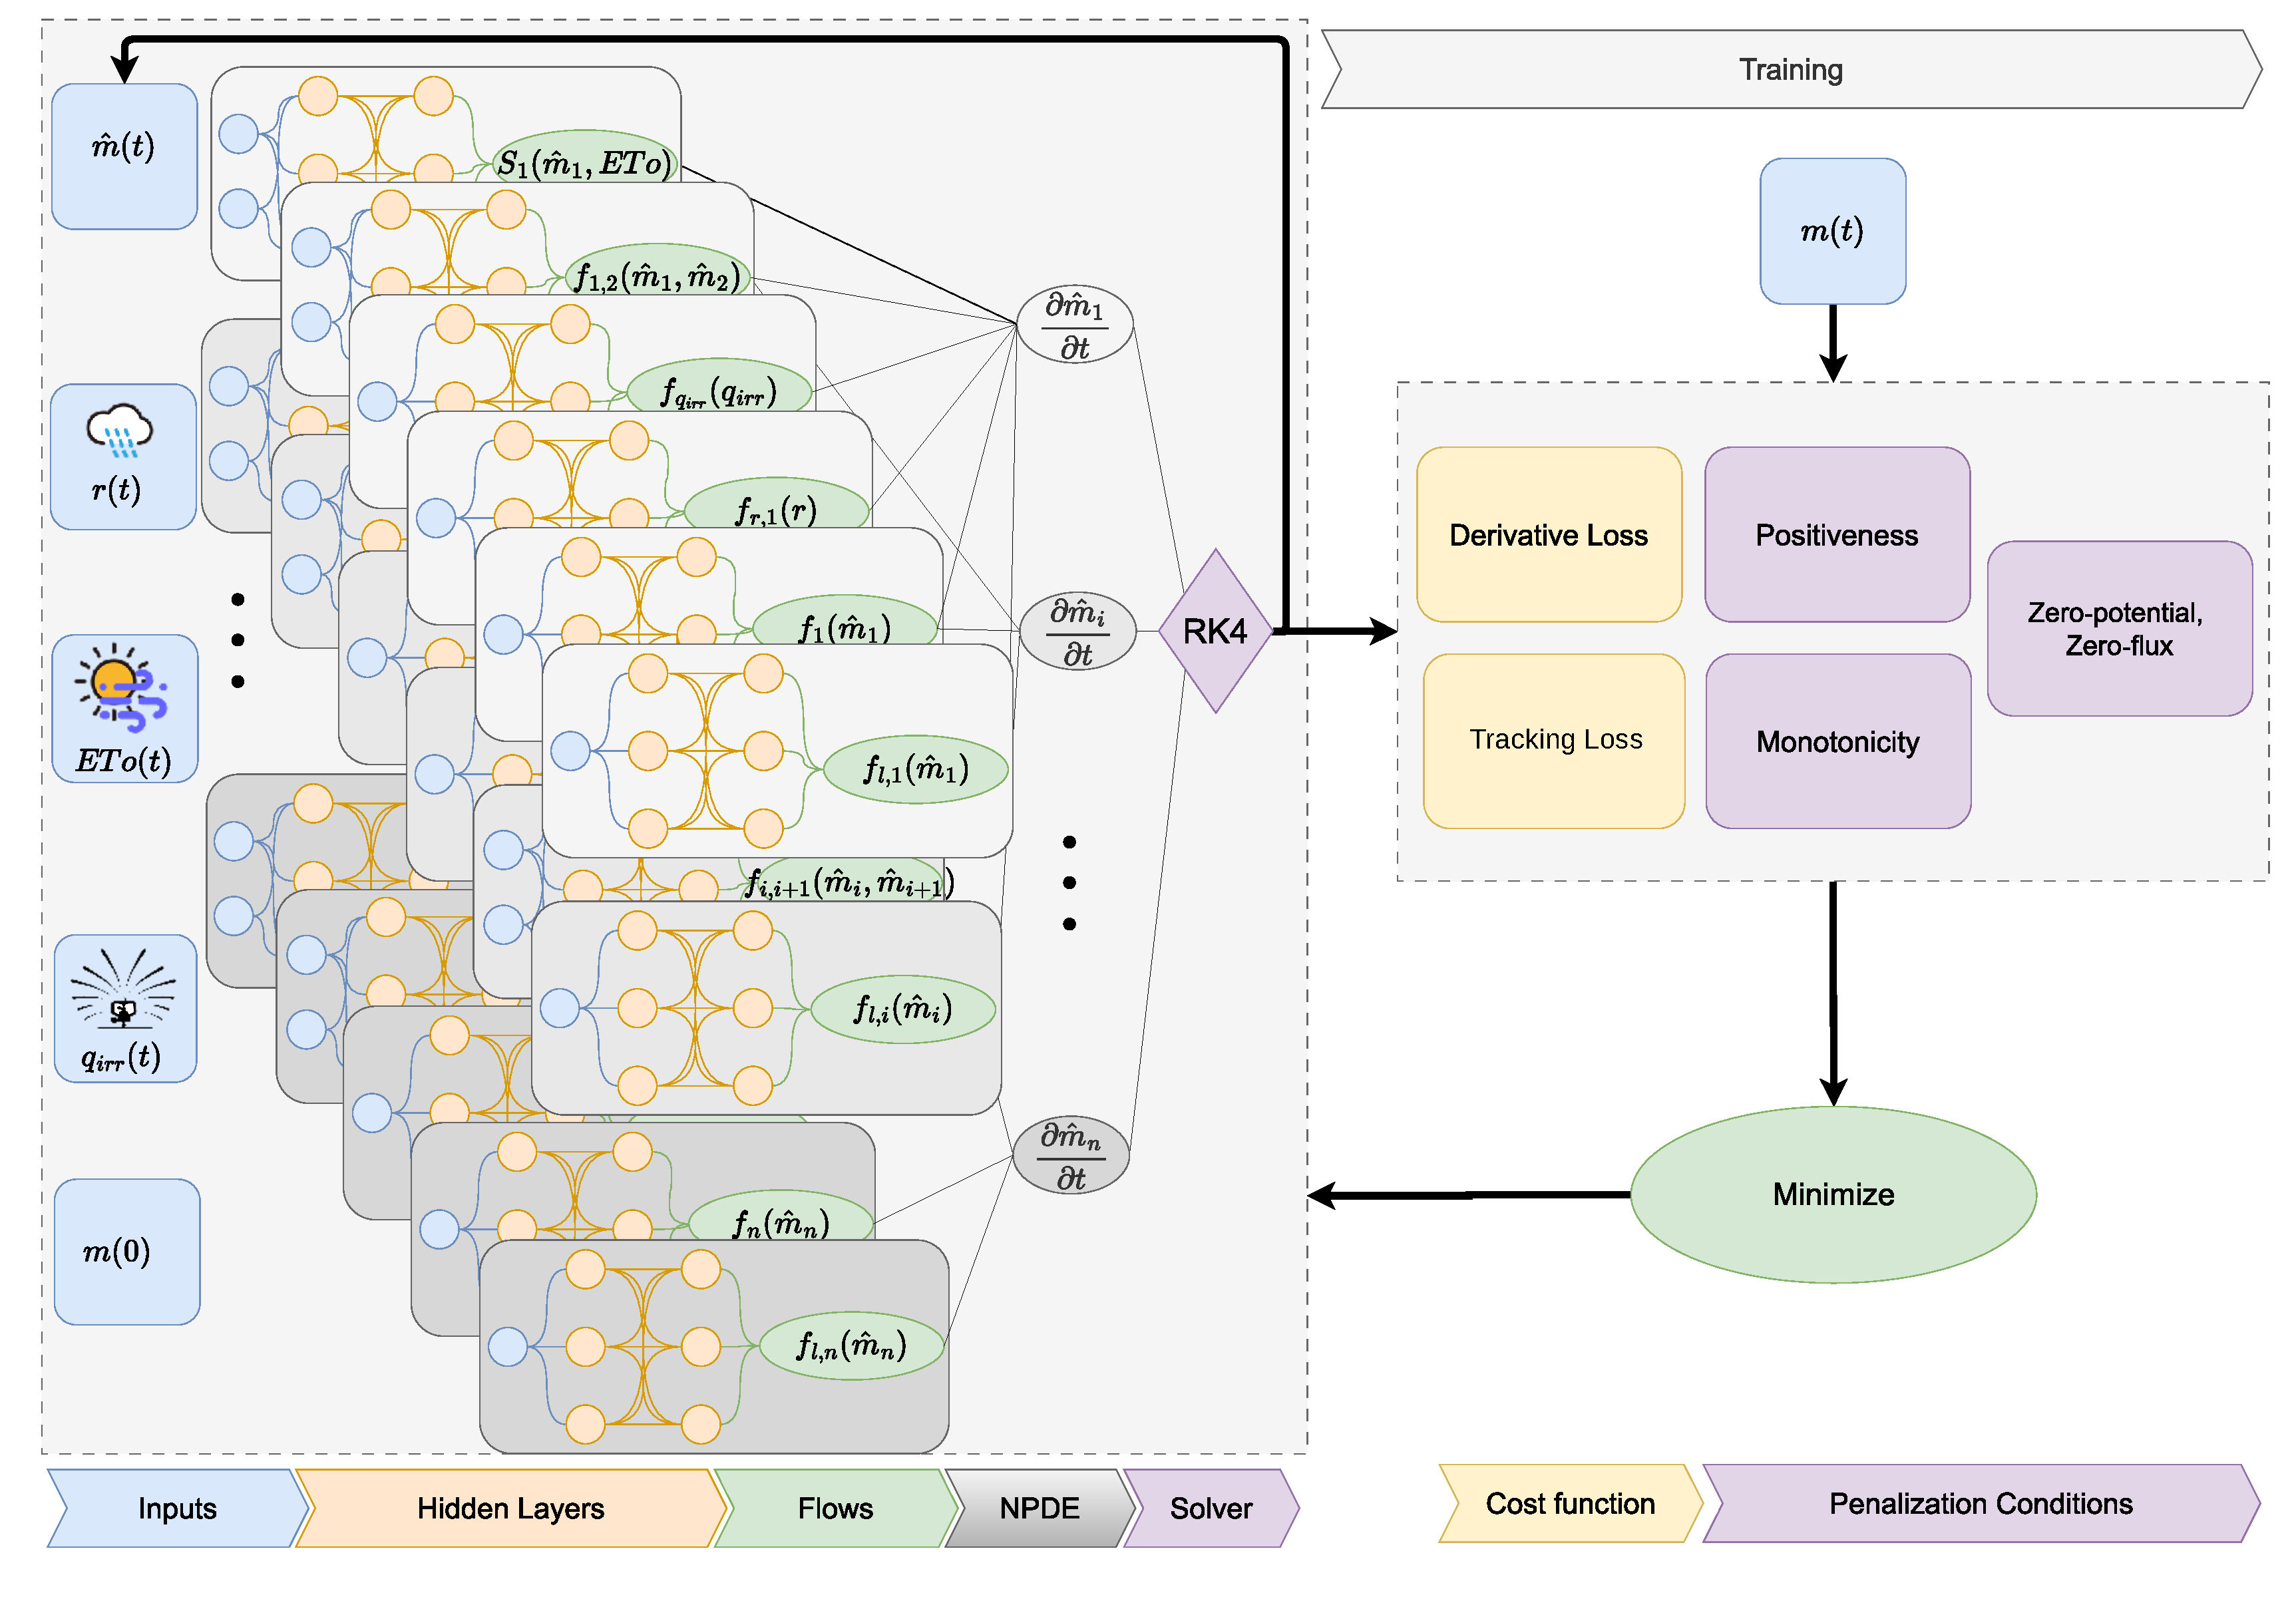
\includegraphics[width=0.90\linewidth]{PINNsmb.pdf}
\setcounter{figure}{4}
\captionof{figure}{\textcolor{blue}{(Revised manuscript) Architecture and two-stage training workflow of the proposed PINN. Inputs comprise the 6-layer moisture vector $\hat{m}(t)$ (5--55~\si{cm}), irrigation ($q_{\mathrm{irr}}$), rainfall ($r$), and reference evapotranspiration ($ET_0$). Inside $g(\hat{m},r,ET_0,q_{\mathrm{irr}},\boldsymbol{\Theta})$, neural branches model vertical drainage $f_i(m_i)$, signed inter-layer exchange $f_{i,i+1}(m_i,m_{i+1})$ ($i=1\dots5$), lateral ditch outflow $fl_i(m_i)$ ($i=1\dots5$; $f_6$ captures lower boundary discharge), rainfall infiltration $fr_i(r)$, surface irrigation $fq_{\mathrm{irr}}(q_{\mathrm{irr}})$, and evapotranspirative sink $S_i(m_i,ET_0)$ ($pc_i$). Stage~1 minimizes derivative loss $j_1$ and Stage~2 refines $\boldsymbol{\Theta}$ via RK4 trajectory tracking loss $j_2$, subject to soft penalties $c_1$--$c_3$.}}
\end{minipage}
\end{center}

\query[R-1.7]{[fig.3] The last column mixes the irrigation plot and the ``row labels'' (``Estimated Flows at 15cm'' etc.). Even if it is difficult to squeeze all these columns in a figure, maybe a scientific notation in the ``Lateral outflow'' y-axis tick labels may help gain some space, and maybe putting these ``row labels'' on the left-hand side, shortened to just the centimeters, is enough.}\\
\ans{\textcolor{blue}{Thank you for these practical layout ideas. We regenerated \textbf{Fig.~4} (formerly Fig.~3) placing shortened depth tags (``5 cm'' to ``55 cm'') cleanly along the left margin away from the Irrigation plot and applying scientific y-axis notation to the Lateral outflow column.}}\\
\Rtext{\emph{\textcolor{darkgreen}{See regenerated Fig.~4 and its updated caption below.}}}

\begin{center}
\begin{minipage}{0.96\linewidth}
\centering
\includegraphics[width=0.96\linewidth]{pinn_functions_vertical_by_layer.pdf}
\setcounter{figure}{3}
\captionof{figure}{\textcolor{blue}{(Revised manuscript) Estimated flux branches describing soil-water dynamics across sensor depths (5--55~\si{cm}, labeled along the left margin; formal branch definitions in Section~2.2.1): $fr_i(r)$ is direct rainfall infiltration (\si{\%VWC/h}); $f_i(m_i)$ is gravitational vertical outflow (\si{\%VWC/h}); $f_{i,i+1}(m_i,m_{i+1})$ is signed potential-driven inter-layer exchange (\si{\%VWC/h}); $S_i(m_i,ET_0)$ is evapotranspirative depletion (\si{\%VWC/h}); $fl_i(m_i)$ is lateral ditch outflow (\si{\%VWC/h}, with scientific y-axis notation for compactness); and $fq_{\mathrm{irr}}(q_{\mathrm{irr}})$ is surface sprinkler inflow (\si{\%VWC/h}). Light blue regions denote the measured training moisture bounds at each depth.}}
\end{minipage}
\end{center}

\query[R-1.8]{[fig.2] The boxplot needs more vertical space, and the heatmap may be enhanced by using a dark frame to separate the white of the plot (0 error) from the white background.}\\
\ans{\textcolor{blue}{We implemented both visual improvements in \textbf{Fig.~2}, adding black rectangular borders around the training and forecasting residual heatmaps and expanding the vertical height of the boxplot panel.}}\\
\Rtext{\emph{\textcolor{darkgreen}{In Fig.~2, the estimation error is distributed around zero during training and forecasting, where the box plots show medians near zero and interquartile ranges below \SI{2.5}{\%VWC} across all depths, with occasional outliers due to the conservative peak response of the PINN.}}}

\begin{center}
\begin{minipage}{0.94\linewidth}
\centering
\includegraphics[width=0.95\linewidth]{error_analysis_heatmap_boxplot.pdf}
\setcounter{figure}{1}
\captionof{figure}{\textcolor{blue}{(Revised manuscript) Soil moisture prediction residuals ($m_i - \hat{m}_i$, \si{\%VWC}) across 5--55~\si{cm} during the 35-day training and 3-day held-out forecasting periods. Black frames delineate heatmap boundaries against zero-error white regions ($-2.5$ to $11.1$~\si{\%VWC}; red under-prediction, blue over-prediction). Bottom boxplots show near-zero medians and interquartile ranges below 2.5~\si{\%VWC} across all depths.}}
\end{minipage}
\end{center}

\query[R-1.9]{[eq.13] In the summation, $t_k$ is both the running index and the extreme element, maybe you can sum over $j = k-n_e+1$ to $k$, and use $t_j$ in the equation.}\\
\ans{\textcolor{blue}{Thank you for catching this notation clash. We updated both stage losses ($j_1$ and $j_2$) and the finite-difference definitions in Sections~2.2.3 and~2.2.4 to sum over $j = k - n_e + 1$ to $k$ with time instants $t_j$, reserving $t_k$ exclusively for the upper window boundary.}}\\
\Rtext{\emph{\textcolor{darkgreen}{\begin{gather*}
    j_{1}(\boldsymbol{\Theta}) = 
    \frac{1}{n_e} \sum_{j = k - n_e + 1}^{k} 
    \left\| 
         \left( 
            \Delta m(t_j) - g(m(t_j), r(t_j), ET_0(t_j), q_{\mathrm{irr}}(t_j), \boldsymbol{\Theta}) 
        \right) 
    \right\|_{\mathbf{W}_1}^2, \\
    j_{2}(\boldsymbol{\Theta}) = 
    \frac{1}{n_e} \sum_{j = k - n_e + 1}^{k} 
    \left\| 
         \mathbf{W}_2^{1/2}\left( 
            m(t_j) - \hat{m}(t_j) 
        \right) 
    \right\|_{1}.
\end{gather*}}}}

\query[R-1.10]{[fig.5] $q_{\mathrm{irr}}$ instead of $q\mathrm{irr}$ (or $q\_\mathrm{irr}$).}\\
\ans{\textcolor{blue}{Thank you. We standardized all occurrences across \textbf{Fig.~7} (formerly Fig.~5), all figure captions, equations, and main text to $q_{\mathrm{irr}}$.}}\\
\Rtext{\emph{\textcolor{darkgreen}{See updated Fig.~7 and caption below.}}}

\begin{center}
\begin{minipage}{0.75\linewidth}
\centering
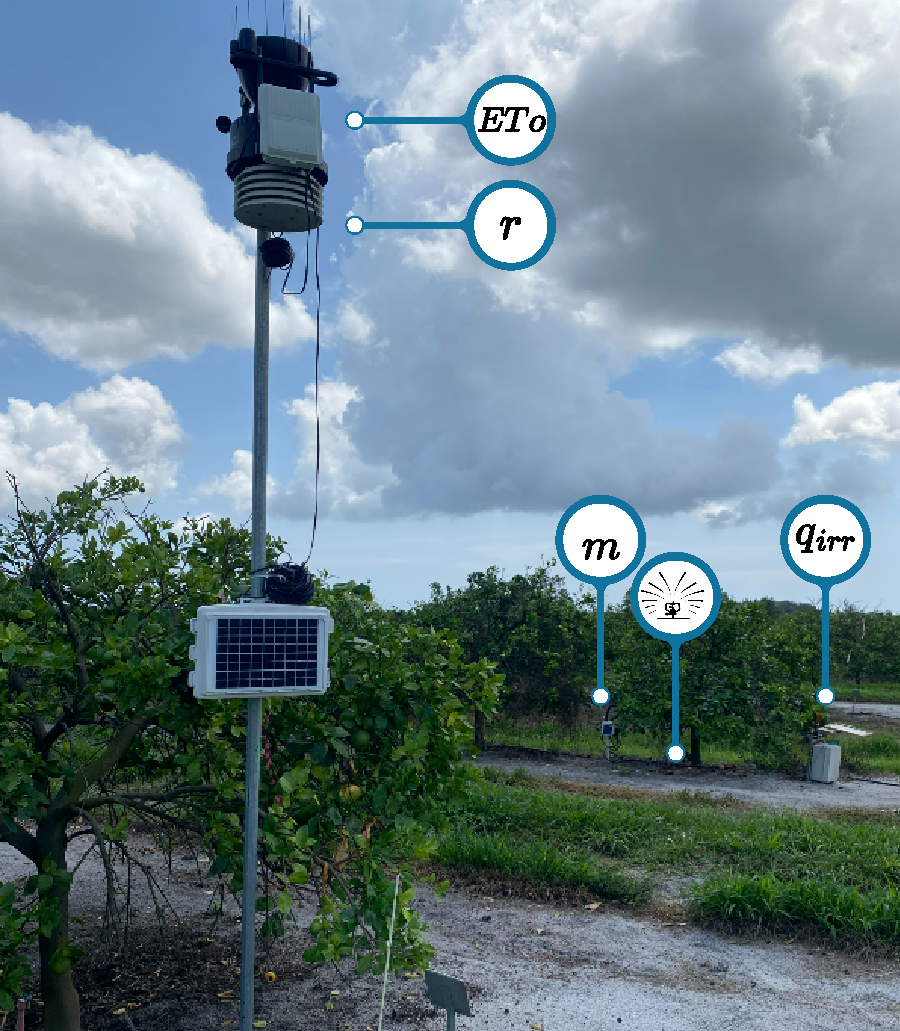
\includegraphics[width=0.58\linewidth]{sensorsmillenniumb.pdf}
\setcounter{figure}{6}
\captionof{figure}{(Revised manuscript) Description of experimental setup, where a weather station, soil moisture probe, and irrigation sensor were deployed to collect soil moisture ($m$), rain ($r$), potential evapotranspiration ($ET_0$), and irrigation (\textcolor{blue}{$q_{\mathrm{irr}}$}) data.}
\end{minipage}
\end{center}

\section*{Answers to Reviewer 2}

\query[R-2.General]{The manuscript presents an interesting and practically relevant approach to soil moisture prediction by integrating physical principles with neural network modeling. The proposed framework is well structured, and the results are promising for precision irrigation applications. Overall, I find the study valuable and potentially suitable for publication in Scientific Reports. I have provided 12 constructive comments in the attached review report, mainly concerning methodological clarification, interpretation of results, and minor presentation improvements. I encourage the authors to address these points in a revised manuscript.}\\
\ans{\textcolor{blue}{We sincerely thank Reviewer~2 for the positive appraisal of our manuscript and for the 12 clear, constructive suggestions, all of which we have addressed in full below.}}

\query[R-2.1]{\textbf{1. Positioning of the contribution:} The Introduction discusses related PINN studies on Richards' equation and soil moisture prediction (Refs.~12--15). It would be helpful to state more explicitly which elements are new in the present study, particularly the sensor-depth discretization, interpretable flux branches, and two-stage training procedure. A concise comparison would help readers identify the main contribution.}\\
\ans{\textcolor{blue}{Thank you for this suggestion. We expanded our positioning relative to recent Richards' PINN surrogates, operator networks, sequence/assimilation forecasters, and lumped water-balance controllers~\cite{Bandai2022, Lan2024, Elkha2024, Bandai2024, Ye2025, WangY2023, ZhangT2025, Bagheri2025, Jiang2025, Jiang2026}, added \textbf{Table~1} (reproduced below), and structured the closing paragraph of the Introduction explicitly around our three methodological elements (First, sensor-depth discretization without prescribed retention curves; Second, decomposed, physically regularized neural flux branches; Third, two-stage derivative-to-RK4 training).}}\\
\Rtext{\emph{\textcolor{darkgreen}{First, we use Richards' equation as a structural framework, spatially discretizing it at sensor depths throughout the soil profile without prescribed soil-retention curves to obtain differential equations that describe the dynamics and relationships of each soil layer with irrigation ($q_{\mathrm{irr}}$), rainfall ($r$), and potential evapotranspiration ($ET_0$), as flow functions that satisfy water balance constraints. Evapotranspirative water depletion appears as a sink function of $ET_0$ and soil moisture at each layer. Second, all flow functions are approximated using decomposed neural network branches that are regularized for physical consistency (non-negativity, monotonicity, and zero-forcing zero-flux). Third, the PINN is trained in two stages: initially, it minimizes errors against measured soil moisture variations, followed by tuning through the incorporation of the fourth-order Runge--Kutta (RK4) numerical solution into the cost function.}}}

\begin{center}
\begin{minipage}{0.98\linewidth}
\centering
\renewcommand{\theHtable}{r2.\arabic{table}}
\setcounter{table}{0}
\captionof{table}{\textcolor{blue}{(Revised manuscript) Comparison of modeling families against the five core requisites for multi-depth predictive irrigation management.}}
\scriptsize
\setlength{\tabcolsep}{3.5pt}
{\color{blue}\begin{tabular*}{\linewidth}{@{\extracolsep{\fill}}>{\raggedright\arraybackslash}p{0.27\linewidth}>{\raggedright\arraybackslash}p{0.16\linewidth}ccccc@{}}
\toprule
\textbf{Modeling Family} & \textbf{Studies} & \textbf{Multi-} & \textbf{No Soil-} & \textbf{Explicit} & \textbf{Depth} & \textbf{Physically} \\
 & & \textbf{Depth} & \textbf{Curve} & \textbf{Irrig.} & \textbf{Fluxes \&} & \textbf{Consistent} \\
 & & \textbf{Profile} & \textbf{Calib.} & \textbf{Input} & \textbf{Depletion} & \textbf{Control} \\
\midrule
Analytical Richards' PDE models & \cite{Celia1990, swap2024} & $\checkmark$ & $\times$ & $\checkmark$ & $\checkmark$ & Partial$^{\mathrm{a}}$ \\
Physics-informed PDE \& operator surrogates & \cite{Bandai2022, Lan2024, Elkha2024, Bandai2024, Ye2025} & $\checkmark$ & Partial & $\times$ & $\times$ & $\times$ \\
Data-driven time-series \& ML forecasters & \cite{Zou2010, Murcia2024, Bagheri2025} & Partial & $\checkmark$ & $\times$ & $\times$ & $\times$ \\
Physics-guided sequence \& assimilation models & \cite{WangY2023, ZhangT2025, Jiang2025, Jiang2026} & $\checkmark$ & $\times$ & $\times$ & $\times$ & $\times$ \\
Control-oriented lumped water balance & \cite{condeforecast2024} & $\times$ & $\checkmark$ & $\checkmark$ & Partial$^{\mathrm{b}}$ & $\checkmark$ \\
\midrule
\textbf{Proposed sensor-depth PINN} & \textbf{This study} & \boldmath$\checkmark$ & \boldmath$\checkmark$ & \boldmath$\checkmark$ & \boldmath$\checkmark$ & \boldmath$\checkmark$ \\
\bottomrule
\end{tabular*}}
\vspace{2pt}
{\footnotesize\color{blue}\raggedright
$^{\mathrm{a}}$Physically consistent, but iterative nonlinear PDE solving is computationally demanding for online MPC.\par
$^{\mathrm{b}}$Separates lumped rainfall, evapotranspiration, and drainage gains, but without vertical depth localization.\par}
\end{minipage}
\end{center}

\query[R-2.2]{\textbf{2. Flux sign conventions and boundary conditions:} In Section~2.2.1, please recheck the sign convention for the downward-positive vertical axis and water flux when moving from Eqs.~(1)--(2) to Eqs.~(3)--(5). A short explanation of the flux directions and the assumed upper and lower boundary conditions would make the derivation and the subsequent model interpretation easier to follow.}\\
\ans{\textcolor{blue}{Thank you for prompting this careful check. In Section~2.2.1, we verified all signs for downward-positive depth $z$ and total head $H = h(m) - z$, fixing the gravity sign in Eq.~(1) so that downward Darcy--Buckingham flux $q = -K(m)\partial H/\partial z = K(m)(1 - \partial h/\partial z)$ and continuity $\partial m/\partial t = -\partial q/\partial z$ yield Eq.~(4) consistently under upstream interface differencing. We also added explicit upper and lower column boundary statements and clarified the flux sign conventions for $f_i(m_i) \ge 0$ and signed $f_{i,i+1}(m_i, m_{i+1})$.}}\\
\Rtext{\emph{\textcolor{darkgreen}{For downward-positive depth $z$ and total hydraulic head $H = h(m) - z$, Richards' equation is $\frac{\partial m}{\partial t} = \frac{\partial}{\partial z}\left[K(m)\left(\frac{\partial h(m)}{\partial z} - 1\right)\right]$. [...] Defining $q$ as a downward water flux, $\frac{\partial m}{\partial t} = -\frac{\partial q}{\partial z}$, the Darcy--Buckingham law is $q = -K(m)\frac{\partial H}{\partial z} = K(m)\left(1 - \frac{\partial h(m)}{\partial z}\right)$. Evaluating upstream $K(m_i)$ and $-\partial h/\partial z \approx (h(m_i)-h(m_{i+1}))/\Delta z$ across the interface between layers $i$ and $i+1$, $q_i = K(m_i)\left(\frac{h(m_i)-h(m_{i+1})}{\Delta z}+1\right)$. [...] At the column boundaries, the surface layer ($i=1$) receives rainfall and sprinkler irrigation minus surface evaporative losses, while the bottom compartment ($i=n$, centered at \SI{55}{cm} and spanning to \SI{60}{cm} depth) discharges vertically via $f_n(m_n)$. [...] Here $f_i(m_i) \ge 0$ represents downward gravitational drainage and $f_{i,i+1}(m_i, m_{i+1})$ represents signed potential-driven exchange (positive downward when $m_i > m_{i+1}$ and negative upward for capillary rise when $m_{i+1} > m_i$).}}}

\query[R-2.3]{\textbf{3. Meaning of the three-day forecast:} Please specify whether rainfall and potential evapotranspiration inputs used during the held-out forecasting period were observed values or actual weather forecasts (Fig.~1 and Section~2.3). This distinction is important for understanding the reported three-day prediction accuracy and how it might translate to operational irrigation scheduling.}\\
\ans{\textcolor{blue}{Thank you for highlighting this distinction. We now state explicitly in the Abstract, Section~1 (Fig.~1 caption and text), Conclusions, and Section~2.3 that held-out evaluations use observed weather-station rainfall ($r$), $ET_0$, and irrigation ($q_{\mathrm{irr}}$) to isolate intrinsic model dynamics, whereas operational scheduling replaces station weather with forecast feeds~\cite{NWS2024}.}}\\
\Rtext{\emph{\textcolor{darkgreen}{Held-out evaluations use observed station rainfall ($r$), $ET_0$, and irrigation ($q_{\mathrm{irr}}$) to isolate intrinsic model dynamics, whereas operational deployment replaces station weather with forecast feeds~\cite{NWS2024}.}}}

\query[R-2.4]{\textbf{4. Consistency of the reported study dates:} Section~2.3 describes the training period as 864 hours (36 days), from 28 March 2025 at 20:00 to 2 May 2025 at 20:00. These timestamps appear to span 840 elapsed hours (35 days). Please verify the dates or duration, and briefly explain the interval between the stated end of training and start of validation, including how the validation initial state was selected.}\\
\ans{\textcolor{blue}{Thank you for catching this discrepancy. The merged training dataset comprises 840 hourly records spanning 839 elapsed hours ($\approx 35$~days) from March~28, 2025, 21:00:00 to May~2, 2025, 20:00:00 (rather than 864~\si{h} / 36~days in the initial draft). Validation comprises 73 hourly records spanning 72 elapsed hours from May~3, 2025, 21:00:00 to May~6, 2025, 21:00:00, leaving a 25-hour separation buffer so the initial state $m(0)$ (measured on May~3 at 21:00:00) is temporally decoupled from training, while all 792 unseen hours through June~5, 2025 are evaluated in Section~1.1.}}\\
\Rtext{\emph{\textcolor{darkgreen}{We collected 840 hourly records spanning 839 elapsed hours ($\approx 35$~days) of data from March 28, 2025, 21:00:00 to May 2, 2025, 20:00:00, for training. [...] Additionally, we extracted 72 elapsed hours (3 days, 73 hourly records) of data from May 3, 2025, 21:00:00 to May 6, 2025, 21:00:00, for validation (leaving a 25-hour separation buffer before the May~3 21:00:00 initial state $m(0)$, with the full 792 unseen hours through June~5, 2025 evaluated in Section~1.1).}}}

\query[R-2.5]{\textbf{5. Depth-specific interpretation of predictive performance:} The overall forecast RMSE and $R^2$ in Table~1 are encouraging, but $R^2$ is negative at 25, 45, and 55\,cm, with particularly large negative values at the two deepest levels. The authors already note the limited variability at these depths. A little more explanation of this effect, and a reminder that the pooled $R^2$ does not represent every layer equally well, would provide a more balanced interpretation.}\\
\ans{\textcolor{blue}{We agree and expanded Section~1 alongside Table~2 (shown in R-1.3a) and Fig.~3 (shown in R-1.3c) to report per-layer $\sigma_m$, explain how dividing small offset errors (\SI{0.95}{} and \SI{1.32}{\%VWC}) by near-zero subsoil variance ($\sigma_m = 0.34$ and \SI{0.17}{\%VWC}) yields negative single-layer $R^2_i$ despite positive correlations ($r = 0.709$ and $0.713$), and remind readers to interpret overall $R^2$ alongside per-layer RMSE and $r$.}}\\
\Rtext{\emph{\textcolor{darkgreen}{Dividing squared error by near-zero variance ($R^2_i = 1 - \mathrm{MSE}_i/\sigma_{m,i}^2$) turns small offset biases at 45 and 55~\si{cm} (\SI{0.95}{} and \SI{1.32}{\%VWC}) into strongly negative single-layer $R^2$ values despite positive correlations ($r = 0.709$ and $0.713$). Therefore, the negative values indicate that at such depths there is low data variability and that the measured data could be better explained by the average than by the model, so overall $R^2$ should be interpreted alongside per-layer RMSE and $r$.}}}

\query[R-2.6]{\textbf{6. Interpretation of the inferred uptake terms:} The estimated depth-specific sink functions are potentially useful, but their identification as plant or root water uptake deserves slightly more qualification. As discussed in the Results, evaporation and drainage-related processes may also contribute to the inferred terms. Please clarify this distinction when discussing the apparent uptake maximum around 25\,cm and avoid implying direct validation of root activity where it was not measured.}\\
\ans{\textcolor{blue}{Thank you for emphasizing this distinction. Throughout the manuscript, we replaced ``plant water uptake'' with \emph{evapotranspirative water depletion} ($pc_i$, denoted $S_i(m_i, ET_0)$ in Section~2.2.1), explicitly qualifying in Sections~1 and~1.2 that $S_i$ captures total $ET_0$-correlated drying (surface evaporation at 5~\si{cm}, root-zone extraction peaking near 25~\si{cm} above the $\approx\SI{30}{cm}$ clay horizon, and unverified daytime ditch/water-table drawdown at 55~\si{cm}) rather than directly measured physiological transpiration.}}\\
\Rtext{\emph{\textcolor{darkgreen}{Elevated depletion rates are estimated at the first layer (5~\si{cm}) and the lowest layer (55~\si{cm}), but these should not be interpreted as root uptake alone. Surface evaporation may contribute at 5~\si{cm}. At 55~\si{cm}, below the shallow root zone, evaporation from the adjacent ditch may draw water from the surrounding soil (Section~2.3), producing an $ET_0$-related moisture loss. This mechanism has not been independently verified. Among the subsurface layers above the \SI{30}{cm} clay horizon, greater depletion is estimated at 25~\si{cm} than at 15~\si{cm}, suggesting a possible peak root uptake zone (Section~1.2).}}}

\query[R-2.7]{\textbf{7. Sampling near zero for the zero-flow penalty:} Section~2.2.6 applies the zero-flow penalty using random synthetic inputs and a very small threshold ($\epsilon = 10^{-7}$). Could the authors clarify whether exact zero or near-zero inputs were deliberately included among the constraint samples? This small detail would help readers understand how the zero-flow condition is enforced in practice.}\\
\ans{\textcolor{blue}{Thank you for pointing this out. In the original draft, $c_3$ was mistakenly grouped with $c_1$ and $c_2$ under the $M = 1{,}000$ random uniform samples (and written with $\epsilon = 10^{-7}$). In practice, the zero-flow condition is enforced in two ways: (i) all branches in $\mathcal{G}_0$ omit bias terms ($\mathbf{b}^{(\ell)} = \mathbf{0}$) and use zero-preserving activations ($\operatorname{mish}(0) = \tanh(0) = 0$), so single-input branches satisfy $g(0) = 0$ by construction (including at $m_i = 0$) and two-input branches satisfy $g(0,0) = 0$; and (ii) unlike $c_1$ and $c_2$, $c_3$ is evaluated across the $n_e = 839$ observed hourly training steps with threshold $|\text{var}| \le \epsilon = 10^{-6}$, where exact zeros occur naturally in field inputs ($r = 0$, $q_{\mathrm{irr}} = 0$, and nighttime $ET_0 = 0$). In particular, this penalizes two-input sinks $S_i(m_i, 0)$ during nighttime hours when $ET_0 = 0$ even though $m_i > 0$. Sections~2.2.2 and~2.2.6 have been clarified accordingly.}}\\
\Rtext{\emph{\textcolor{darkgreen}{Because all branches in $\mathcal{G}_0$ omit bias terms ($\mathbf{b}^{(\ell)} = \mathbf{0}$) with $\operatorname{mish}(0) = \tanh(0) = 0$, single-input branches satisfy $g(0) = 0$ by construction, while two-input branches satisfy $g(0,0) = 0$. Complementing this, the term $c_3$ promotes that flux functions, such as drainage or irrigation, are zero when their driving variables (e.g., soil moisture or irrigation rate) are zero or nearly zero, as no flow should occur without a driving force. [...] Here $g(\mathbf{x}_s)$ is the flux evaluated across the $n_e = 839$ observed hourly steps of the training window (rather than the random synthetic draws used in $c_1$ and $c_2$), and $\delta_s = 1$ if the driving variable (e.g., soil moisture for $f_i$, $|m_i - m_{i+1}|$ for $f_{i,i+1}$, or either soil moisture or $ET_0$ for $S_i$) satisfies $|\text{var}| \le \epsilon = 10^{-6}$, and $\delta_s = 0$ otherwise. In field records, exact zeros occur regularly in external inputs ($r = 0$, $q_{\mathrm{irr}} = 0$, and nighttime $ET_0 = 0$), allowing $c_3$ to penalize two-input sinks $S_i(m_i, 0)$ when $ET_0 = 0$ even though $m_i > 0$.}}}

\query[R-2.8]{\textbf{8. Interpretation of soft physical constraints:} The non-negativity and monotonicity penalties are valuable design features. However, Fig.~3 and the accompanying discussion acknowledge a small negative/non-monotonic lateral-flow behavior. It would be useful to state explicitly that finite penalty terms encourage, rather than strictly guarantee, the prescribed properties, and briefly explain how signed inter-layer flows are treated in this framework.}\\
\ans{\textcolor{blue}{We agree completely and clarified in Section~1 (discussing $fl_5$), Section~2.2, and Section~2.2.6 that finite multipliers ($\lambda_{c_1}, \lambda_{c_2}, \lambda_{c_3}$) act as \emph{soft physical regularizers} that strongly promote rather than algebraically force positivity and monotonicity, while $f_{i,i+1}$ and $f_n$ are excluded from $c_1$ to allow signed bidirectional capillary exchange and lower-boundary discharge (while still entering the monotonicity set $\mathcal{D}$ in $c_2$).}}\\
\Rtext{\emph{\textcolor{darkgreen}{Because these enter through finite multipliers ($\lambda_{c_1}, \lambda_{c_2}, \lambda_{c_3}$), they act as \emph{soft physical regularizers} that strongly promote, rather than algebraically force, these properties. [...] Note that $f_n$ and inter-layer terms $f_{1,2},\dots,f_{n-1,n}$ are excluded, as their flow direction depends on boundary or bidirectional potential gradients ($m_i \gtrless m_{i+1}$).}}}

\query[R-2.9]{\textbf{9. Additional implementation details:} For reproducibility, please consider adding a concise account of how input normalization to $[0, 1]$ was implemented, the numerical time step used with RK4, and the principal settings for the second training stage. Where applicable, reporting how the random sampling of constraint points was controlled would also be helpful. These descriptions would complement the shared datasets/inference code without requiring release of proprietary training software.}\\
\ans{\textcolor{blue}{Thank you. We added all implementation settings in Sections~2.2.2, 2.2.3, 2.2.4, and~2.4: fixed $[0,1]$ normalization divisors ($m/40\,\si{\%VWC}$, $q_{\mathrm{irr}}/1.0\,\si{h/h}$, $r/30\,\si{mm/h}$, $ET_0/0.8\,\si{mm/h}$), per-branch activations and widths (\texttt{mish}/\texttt{tanh}, $H=56$, $2H=112$ on $S_i$, 375,089 parameters), hourly RK4 step ($\Delta t = \SI{1}{h}$), fixed seed \texttt{42} for initialization and $M=1{,}000$ uniform collocation draws, and AMSGrad-Adam schedules (clipping at 0.5, decay 0.9 every 1,000 steps; Stage~1: 3,000 epochs from $\eta_1 = \num{7.97e-5}$; Stage~2: 1,000 epochs from $\eta_2 = \num{5.0e-6}$), alongside full open code release on Zenodo.}}\\
\Rtext{\emph{\textcolor{darkgreen}{All input data (e.g., soil moisture, irrigation, rainfall, and evapotranspiration) are normalized to $[0, 1]$ using fixed operational bounds ($m/40\,\si{\%VWC}$, $q_{\mathrm{irr}}/1.0\,\si{h/h}$, $r/30\,\si{mm/h}$, and $ET_0/0.8\,\si{mm/h}$, with $\Delta t = \SI{1}{h}$). [...] Randomness across initialization and uniform collocation sampling ($M = 1{,}000$ points per step) was controlled using fixed seed \texttt{42} across Python, NumPy, and TensorFlow. Both stages used AMSGrad-Adam optimization with gradient norm/value clipping at 0.5 and staircase exponential decay (factor 0.9 every 1,000 steps): Stage~1 ran for 3,000 epochs starting from $\eta_1 = \num{7.97e-5}$, and Stage~2 refined parameters via RK4 trajectory tracking for 1,000 epochs starting from $\eta_2 = \num{5.0e-6}$.}}}

\query[R-2.10]{\textbf{10. Context for the reported forecast error:} The overall forecasting RMSE is promising. If an existing persistence estimate or similarly simple reference result can be obtained readily from the current data, a brief comparison would help contextualize the result. If not, a short qualitative discussion of accuracy relative to soil moisture variability and practical sensing requirements would serve the same purpose; new field experiments are not necessary for this clarification.}\\
\ans{\textcolor{blue}{We implemented the Persistence baseline ($\dot{m}=0$) directly on the same training, 3-day test, and 30 rolling unseen 3-day windows in Section~1.1 (Table~3 under R-1.3d above), and contextualized errors against millimeter water depth and capacitive probe tolerances in Section~1 (R-1.3a). Relative to Persistence, the PINN reduces 3-day RMSE by 35.6\% overall (\SI{1.91}{} to \SI{1.23}{\%VWC}; $R^2$ rising from 0.54 to 0.81), cuts dynamic 5~\si{cm} topsoil RMSE by 53.2\% (\SI{4.32}{} to \SI{2.02}{\%VWC}), and lowers 30-window mean 3-day RMSE from $\SI{1.86}{}\pm\SI{1.02}{}$ to $\SI{1.04}{}\pm\SI{0.53}{\%VWC}$.}}\\
\Rtext{\emph{\textcolor{darkgreen}{The full PINN reduces 3-day error by 35.6\% over \textbf{Persistence} (1.91 to 1.23~\si{\%VWC}; 53.2\% in the 5~\si{cm} topsoil, from 4.32 to 2.02~\si{\%VWC}).}}}

\query[R-2.11]{\textbf{11. Scope of generalization and irrigation-control claims:} The field demonstration is based on one citrus site and a short held-out period. Please emphasize this scope when discussing transfer to other soils and crops. It would also improve the Conclusion to distinguish the demonstrated forecasting model from a fully tested model-predictive irrigation controller: water savings and optimized irrigation decisions are promising potential applications, but are not directly evaluated here.}\\
\ans{\textcolor{blue}{We completely agree and dedicated the closing paragraph of the Conclusions section to stating these exact scope boundaries: single-site sandy Alfisol validation over 35 training days and 33 spring test days using observed station meteorology, factory probe calibration, and duration-based irrigation sensing, as well as the explicit distinction between our validated open-loop multi-depth estimator and future closed-loop MPC field trials.}}\\
\Rtext{\emph{\textcolor{darkgreen}{Several limitations define the scope of this study and guide future work. Calibration and validation reflect a single sandy Alfisol citrus block over a 35-day training period and a 33-day spring test period using observed station meteorology, factory probe calibration, and duration-based irrigation sensing; extending the approach to finer-textured soils, other crops, live numerical weather forecasts, and site-specific volumetric calibration requires multi-site, multi-season trials. In addition, the \SI{1}{h} sampling interval matched to forecast providers smooths rapid sub-hourly infiltration peaks in sandy topsoil. Finally, the present work validates an open-loop multi-depth estimator rather than a closed-loop controller; coupling this estimator with operational weather forecasts in field model predictive control trials to measure actual water and nutrient savings is the natural next step.}}}

\query[R-2.12]{\textbf{12. Figures and statistical reporting:} Please clarify what the ``90\% confidence interval'' in the discussion of Fig.~1 refers to and how it was obtained, as the graphical representation is not immediately evident. In Table~1, please identify the statistical test associated with the stated $p$-values. Minor presentation edits, including correcting ``Traking Loss'' in Fig.~4 and improving the legibility of the dense panels in Fig.~3, would also be welcome.}\\
\ans{\textcolor{blue}{Thank you for catching all four presentation details: (i) in \textbf{Fig.~1} and Section~1, we clarified that the 3.5 to 10.2~\si{\%VWC} heatmap color scale is an empirical contrast range (5.8th to 92.1st training percentiles, enclosing 86.3\%, i.e., $\approx 90\%$ of observations) rather than a statistical confidence interval; (ii) in Table~2 (shown in R-1.3a), we identified the two-sided Student's $t$-test associated with the Pearson $r$ $p$-values ($p < 0.0001$, except $^*p = 0.0038$ at 25~\si{cm} in forecasting); (iii) in Fig.~5 (shown in R-1.6), we corrected ``Tracking Loss''; and (iv) in Fig.~4 (shown in R-1.7), we moved shortened centimeter labels to the left margin and formatted lateral outflow y-axes in scientific notation.}}\\
\Rtext{\emph{\textcolor{darkgreen}{The heatmap color scale is clipped to the dominant $\approx 90\%$ empirical moisture range so transient topsoil storm spikes do not saturate contrast across intermediate depths.}}}

\begin{center}
\begin{minipage}{0.96\linewidth}
\centering
\includegraphics[width=0.96\linewidth]{estimation_vs_validation_with_plant_uptake.pdf}
\setcounter{figure}{0}
\captionof{figure}{\textcolor{blue}{(Revised manuscript) Evaluation of the proposed PINN for multi-depth soil moisture prediction, showing measured rainfall ($r$, \si{mm/h}), irrigation duration fraction ($q_{\mathrm{irr}}$, \si{h/h}), reference evapotranspiration ($ET_0$, \si{mm/h}), and measured versus estimated soil moisture (\si{\%VWC}) across 5--55~\si{cm} over the 35-day training period (839~h) and held-out 3-day forecast (72~h, after a 25-h buffer), driven solely by $m(0)$ and observed ($r, q_{\mathrm{irr}}, ET_0$). Moisture heatmaps use a 3.5--10.2~\si{\%VWC} contrast range (5.8th--92.1st training percentiles, enclosing 86.3\% of observations). Lower panels show inferred evapotranspirative depletion rates ($pc_i$, denoted $S_i(m_i,ET_0)$ in Section~2.2.1, \si{\%VWC/h}).}}
\end{minipage}
\end{center}

\vspace{0.3cm}
\bibliographystyle{unsrt}
\bibliography{PINN}

\end{document}
